%\documentclass[master,tocprelim]{Latex/Classes/PhDthesisPSnPDF}
%\documentclass[letterpaper,12pt]{cls/thesis}
%\documentclass[master,final,tocprelim]{unrthesis}
\documentclass[master,tocprelim,12pt]{unrthesis}
%\documentclass[master,tocprelim,12pt]{thesis}

\usepackage{amsmath}
\usepackage{amsthm}
\usepackage{amssymb}
\usepackage{graphicx}
%\usepackage{float}
%\usepackage{wrapfig}
%\usepackage{showkeys}
\usepackage{algorithm2e}
\usepackage{plain}
\usepackage{pdfpages}

\usepackage{listings}

\graphicspath{{./graphics/}}

\lstset{ %
language=C,               
basicstyle=\footnotesize,
showspaces=false,               
showstringspaces=false,         
numbers=left,                   % where to put the line-numbers
numberstyle=\footnotesize,      % the size of the fonts that are used for the line-numbers
stepnumber=1,                   % the step between two line-numbers. If it is 1 each line will be numbered
numbersep=10pt,     
showtabs=false,                 
columns=fullflexible,
frame=single,          
tabsize=2,          
captionpos=b,       
extendedchars=true,
frame=single,
breaklines=true,       
breakatwhitespace=false, 
escapeinside={\%*}{*)}       
}
\def\verbatimtabsize{4\relax}
\def\listingoffset{1em}
\def\listinglabel#1{\llap{\tiny\it\the#1}\hskip\listingoffset\relax}
\def\mylisting#1{{\fontsize{10}{11}\selectfont \listinginput[1]{1}{#1}}}
\def\myoutput#1{{\fontsize{9}{9.2}\selectfont\verbatimtabinput{#1}}}

\newtheorem{proposition}{Proposition}[chapter]
\newtheorem{theorem}{Theorem}[chapter]
\newtheorem{lemma}{Lemma}[chapter]
\newtheorem{corollary}{Corollary}[chapter]
\theoremstyle{definition}
\newtheorem{definition}{Definition}[chapter]
\newtheorem{property}{Property}[chapter]

\title{Dynamical Systems: Chaotic Attractors and \\{~}
    Synchronization using Time-Averaged Partial \\{~}\\
\vskip-12pt
Observations of the Phase Space}
\author{
Jordan Fleming Blocher 
}

%\date{\today}

\newcommand{\cF}{{\mathcal F}}
\newcommand{\cO}{{\mathcal O}}
\newcommand{\cA}{{\mathcal A}}
\newcommand{\cB}{{\mathcal B}}
\newcommand{\cV}{{\mathcal V}}
%\newcommand{\R}{\textbf{R}}
\newcommand{\R}{{\bf R}}
\newcommand{\B}{{\cal B}}
\newcommand{\C}{\textbf{C}}
\newcommand{\del}{\delta}
\newcommand{\cL}{{\mathcal L}}
\newcommand{\mydelta}{{h}}
\newcommand{\yourdelta}{{\Delta}}
\def\words#1{\quad\hbox{#1}\quad}
\def\wwords#1{\qquad\hbox{#1}\qquad}
\renewcommand{\emptyset}{\O}
\numberwithin{equation}{chapter}
\begin{document}

\maketitle

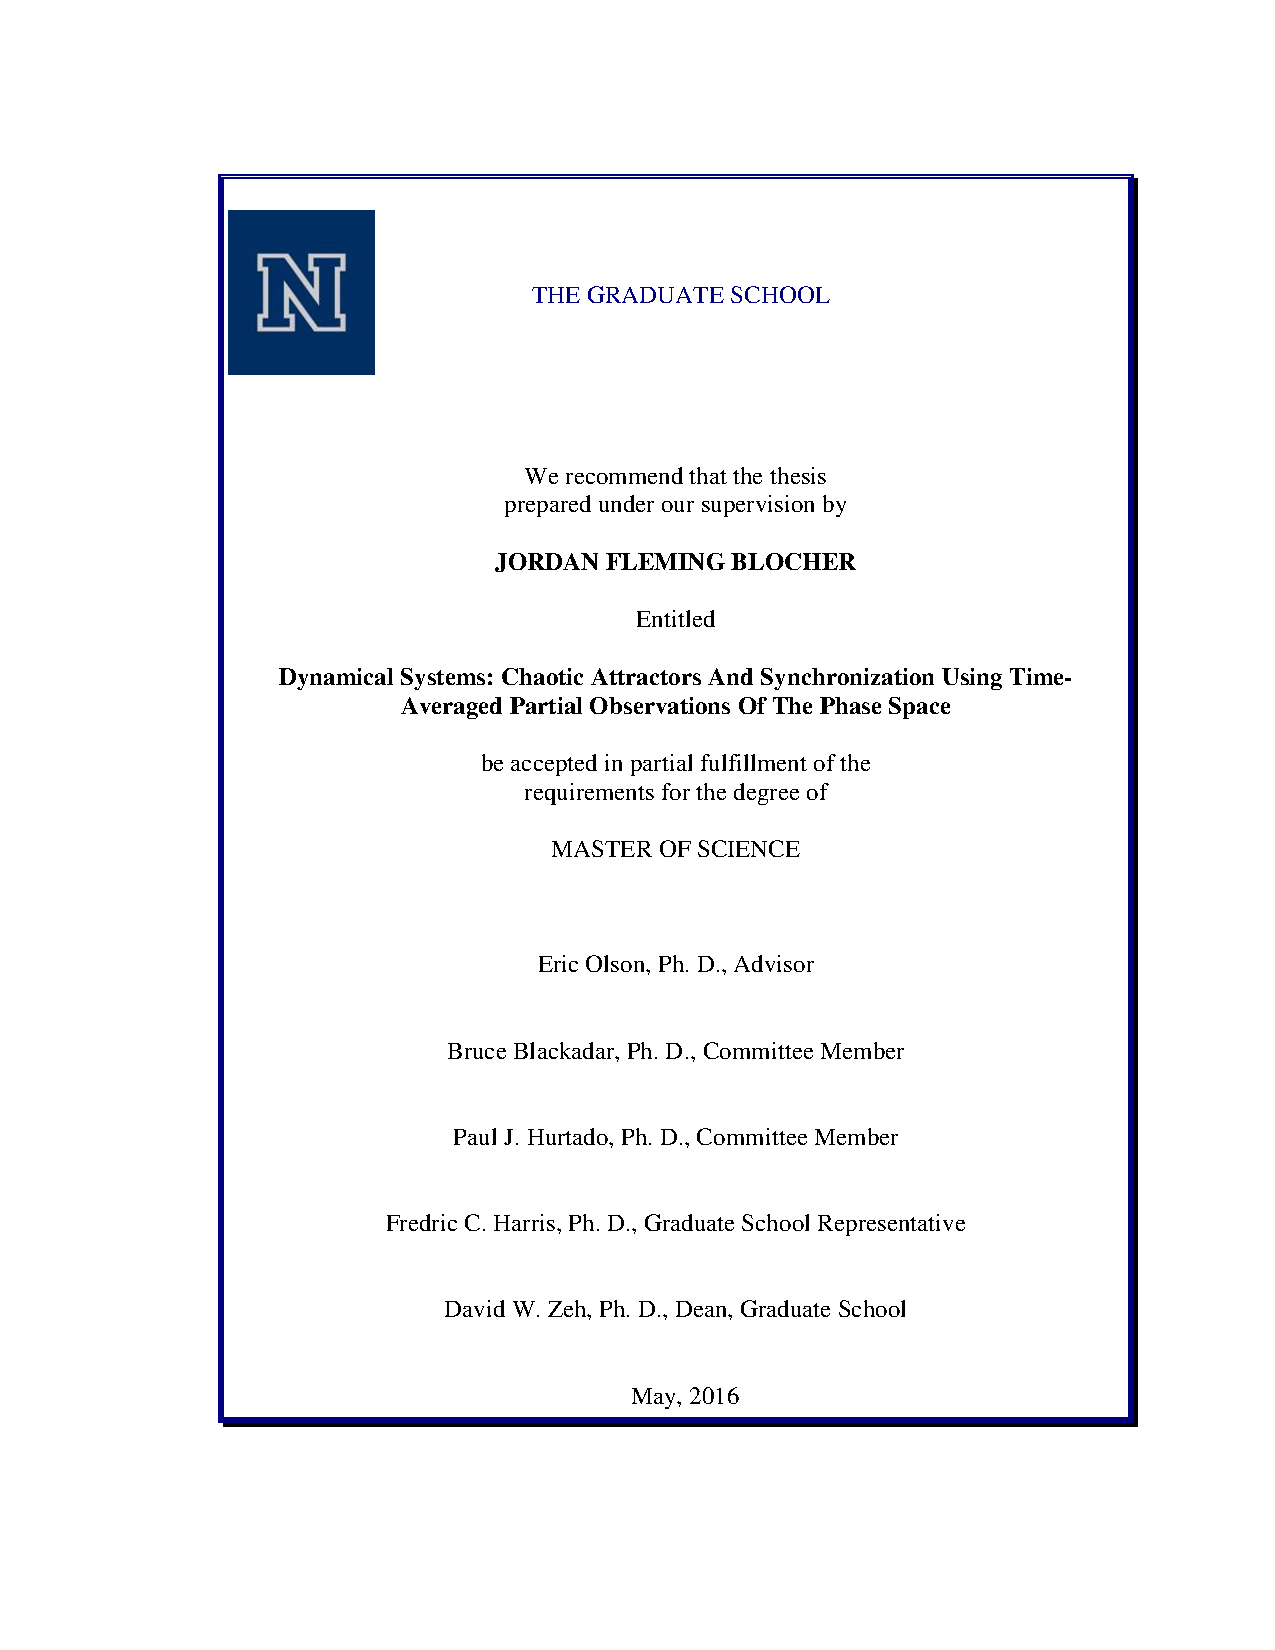
\includepdf{ms-committee-page.pdf}

\begin{abstract}

We study the synchronization of chaotic systems when the coupling
between them contains both time averages and stochastic noise.
Our model dynamics are given by the Lorenz equations
which are a system of three ordinary differential
equations in the variables $X$, $Y$ and $Z$.
Our theoretical results show that coupling two copies of the
Lorenz equations using a feedback control which consists
of time averages of the $X$ variable
leads to exact synchronization provided the
time-averaging window is known and sufficiently small.
In the presence of noise the convergence is to within a
factor of the variance of the noise.
The novelty of our investigation hinges on the
analysis of the time averages.
We also consider the case when the time-averaging window
is not known and show that it is possible to tune the
feedback control to recover the size of the
time-averaging window.
Further numerical computations
show that synchronization is more accurate and occurs
under much less stringent conditions than our theory requires.

\end{abstract}

\begin{acknowledgements}
I would like to acknowledge my thesis advisor, Eric Olson.
I would like to thank my committee members:
Bruce Blackadar, Paul Hurtado and Fred Harris.
I would also like to thank my friends, family and UNR.
This research is supported in part by NSF grant DMS-1418928.
\end{acknowledgements}

\contentspage
\tablelistpage
\figurelistpage

\begin{manuscript}
\chapter{Introduction}\label{Intro}

We produce synchronization results when coupling is applied on 
two chaotic systems when the coupling
between them contains both time averages and stochastic noise.
Our model dynamics are given by the Lorenz equations
which are a system of three ordinary differential
equations in the variables $X$, $Y$ and $Z$.
We build off of investigations of the Lorenz model in 
\cite{Hayden11, Stuart14}, where 
space and continuous time observations \cite{Olson14} by use of a control
theory perspective similar to that which arises from the derivation of
continuous time limits of discrete time filters \cite{ Bloemker14}. 
We seek to determine relationships between the underlying
dynamical system and the observation operator
to ensure that synchronization can be obtained.
For a coupled pair of chaotic dynamical systems,
where the driven system's initialization is not known precisely, the extent 
of the use of observed data over time is a topic of interest in 
meteorology, weather forecasting and any attempt to predict the 
future using incomplete information about the current state of a
dynamical model.

In this thesis, we extend the approach of \cite{Olson14}
to use time-averaged continuous-in-time partial observations of 
the phase space. We examine
both the noise-free case and the case where the observations include
stochastic noise. We are able to show that the use of time-averaged
observations results in synchronization.
The techniques investigated here are applicable to different
dissipative dynamical systems, and
provide many points of continued study, which
are detailed in a chapter dedicated to future work.

The outline of the thesis is as follows. In Chapter 1 we introduce the concept
of synchronization on the global attractor. We also provide a
detailed description of our model problem, a simplified model of atmospheric
convection, the Lorenz system, and present an analytical bound on the
trajectories which is used throughout the thesis. We also introduce the coupling
method that is is the focus of the thesis and introduce the notation that will
be used to describe our experiments.
In Chapter 2 we present a proof of the
existence and uniqueness of our solution. In addition, we present a generalized
Gronwall integration proof that will be used throughout the thesis and is
applicable to the convergence of our model. 
In chapter three we study the convergence of the approximating solution in a noise-free 
setting, ending with an investigation into the sensitivity of the time-averaging
window. Chapter 4 presents an analysis when the observations contain stochastic noise. 
Chapters 5 and 6 present our numerical methods and conclusions. Finally, Chapter
7 provides points of future work.

\section{Synchronization}\label{Synchro}

Synchronization means that the difference between two solution
trajectories converge to zero as time tends to infinity.  The sensitivity
to initial conditions of dynamical systems means that two identical
systems with even a slight perturbation of initial conditions quickly
become uncorrelated even though they are bounded and converging to the
same attractor.  
On the theoretical side, we would like to determine 
when coupling between two identical copies of a dynamical system
leads to synchronization and to study the effects that
realistic conditions, such as a moving time-averages and 
noisy observations, have on the synchronization.
On the computational
side, we would like to simulate the same things and test the
sharpness of our theory.

Consider a dynamical system given by the ordinary differential equations
\begin{equation}\label{freeODE}
    \frac{dU}{dt} = \cF(U) 
\end{equation}
where $U(0) = U_0\in{\bf R}^n$ and ${\cal F}\colon{\bf R}^n\to{\bf R}^n$.
We use partial information about $U$ to drive a second solution $u$
as follows:
\begin{equation}\label{noerra}
    \frac{du}{dt} = \cF(u) + \mu\big(\widetilde{\cal R}(U) - {\cal R}(u)\big)
\end{equation}
with arbitrary initial condition $u(0) = u_0$.
Here $\widetilde{\cal R}(U)$ denotes an interpolation of
partial observations of $U$ back into the phase space ${\bf R}^n$
that may contain noise as well moving time averages, and
${\cal R}(u)$ denotes a feedback control used to nudge $u$
towards $U$ over time.
Note that the relaxation parameter $\mu > 0$ 
determines the rate
at which $u$ is nudged towards $U$ as it evolves forward in time 
and represents a tunable parameter in the system.

Note, we assume the forcing function ${\cal F}$ is known 
exactly and leads to a well posed dynamical system that governs
the freely evolving solution.
More realistically, ${\cal F}$ might only be known up to an
approximation $\widetilde {\cal F}$.  Ideas for work along these 
lines is discussed in Section \ref{whatissigma} in the
chapter on future work.  
We assume the dynamics given by ${\cal F}$ are dissipative.
However, our analysis relies not just on dissipativity, but
on a squeezing property with respect to the observable
part of the phase space.

If $\widetilde{\cal R}={\cal R}$ and $u_0=U_0$, then
$\mu\big((\widetilde{\cal R}(U_0) - {\cal R}(u_0)\big)= 0$.
It follows that both $u$ and $U$ evolve according to the same
dynamics, which in turn implies $u(t)=U(t)$ for all $t\ge 0$.
When $u_0\ne U_0$ it may still happen
%provided $\widetilde{\cal R}={\cal R}$ 
that $\|u(t)-U(t)\|\to 0$ as $t\to\infty$.
When this happens we say that $u$ synchronizes with $U$.
Note, however, when $\widetilde{\cal R}\ne{\cal R}$ it
may happen that
$\mu(\big(\widetilde{\cal R}(U_0) - {\cal R}(u_0)\big)\ne 0$
even if $U_0=u_0$.
It immediately follows that $U(t)\ne u(t)$ for $t>0$.
In this case, we look for bounds on $\|U-u\|$ that depend
on the quality of the approximation $\widetilde{\cal R}\approx{\cal R}$.

If the observations $\widetilde{\cal R}$ have been 
contaminated using a moving time average with a known window size,
then ${\cal R}$ can also include an identical moving time average
so that $\widetilde{\cal R}={\cal R}$.  However, if the size of
the averaging window is unknown, then we can only guess its size.
In this case ${\cal R}$ is only an approximation of $\widetilde{\cal R}$.
Similarly, if the observations $\widetilde{\cal R}$ contain a 
unknown noise term, this this noise can not be included in the 
feedback term and again ${\cal R}$ will differ from 
$\widetilde{\cal R}$, this time by the noise.
The main result of this thesis are theoretical and numerical
bounds on the expected value of $\|U-u\|^2$ in the case 
when $\widetilde{\cal R}$
contains noisy observations that have been averaged with
respect to an unknown window size.



\section{Global Attractors}

For general continuous time dynamical systems the number of degrees of freedom
is often associated with the number of first order ordinary differential
equations (ODEs) in the model.  If
$$ 
\displaystyle\sum_{i=1}^n{\partial \cF_i \over \partial U_i }< 0,
$$
then the system is said to be
\emph{dissipative} system.
This indicates that volumes transported by the dynamics of
the system are contracting.
In this case, there exists a compact set to which all bounded 
sets converge as they are transported by the flow.
In particular, all trajectories eventually converge that set.
Moreover, if this set is invariant, that is, if every point on
the attractor is the image under the flow of the
dynamics over a fixed period of time of another point on the attractor, 
then the set is unique and called the global attractor.
Since the attractor is bounded and invariant, then any trajectory 
on the attractor is bounded backwards in time.
This leads to another characterization of the attractor
as the set of all solutions which are bounded backwards
in time.  
Note that the set of fixed points such that 
$\big\{\, x : {\cal F}(x)=0 \,\big\}$ are included in the attractor,
as is the unstable manifold of the fixed point.
This observation can be used to find lower bounds on the
size of the attractor.


Due to the presence of an attractor, the sum of the Lyapunov
exponents is expected to be negative; an indication that the 
system is dissipative. 
The Lyapunov exponents control the exponential growth or
contraction of volume elements in phase space \cite{Doering95a}.
They 
quantify the exponential divergence of infinitesimally close 
state-space trajectories 
and estimate the amount of chaos in a system. 
A positive exponent is consistent with diagnosing chaos and represents
local instability in a particular direction.

The Lyapunov spectrum is represented geometrically as a small $n$-dimensional 
sphere of initial conditions.
%, where $n$ is the degrees of freedom in the system.
In a chaotic attractor, the sphere evolves into an ellipsoid whose
principal axes expand (or contract) at rates given by the Lyapunov
exponents.
Calculating the largest Lyapunov exponent can yield an estimate 
of the ``level of chaos" using the slope of the divergence
as was calculated by Rosenstein and Collins \cite{Rosenstein93}.
This determines how two trajectories with nearby initial conditions 
diverge over time.
In fact, we expect that two randomly chosen initial 
conditions in arbitrary phase space will diverge exponentially at 
the rate given by the largest Lyapunov exponent. 
In the context of the synchronization studies in this thesis, 
it is this tendency for the
trajectories to diverge that needs to be overcome by the
feedback controller represented by $\mu\big(\tilde{\cal R}(U)-{\cal R}(u)\big)$
in equation~(\ref{noerra}).

\section{The Lorenz '63 Model}

The Lorenz '63 Model is a system of three ordinary differential equations that
represent a simplified model of atmospheric convection \cite{Lorenz63}. 
The model is dissipative with a quadratic energy-conserving nonlinearity.
This system of three coupled non-linear ordinary differential
equations satisfies equation~(\ref{freeODE}) where
$U=(X,Y,Z)$ and
\begin{align}\label{freeLorenz}
    \cF(U)=\begin{bmatrix}\sigma(Y-X)\\
    -\sigma X-Y-XZ\\ -bZ+XY-b(r+\sigma)\end{bmatrix}.
\end{align}
Here $\sigma$ is
the Prandtl number, $r$ is the Rayleigh number, 
and $b$ is a geometric factor. 
Note that we have employed a coordinate system where 
the center is shifted to the point $(0, 0, 0)$.
We will use the standard parameter values 
$\sigma=10$, $b=8/3$ and $r=28$
in our study.  
At these values, the system is known to 
have a chaotic global attractor $\cA$, Tucker \cite{Tucker1999}.

Note that
$$
\displaystyle\sum_{i=1}^3{\partial \cF_i \over \partial U_i }
	=-\sigma-1-b
$$	
which shows the system is dissipative.
Moreover, linearization about the
fixed point $$(\sqrt{b(r-1)},\sqrt{b(r-1)},-\sigma-1)$$
gives the matrix
$$
\begin{bmatrix}
    -\sigma & \sigma & 0\\
    1 & -1 & -\sqrt{b(r-1)}\\
    \sqrt{b(r-1)} & \sqrt{b(r-1)} & -b
\end{bmatrix}.
$$
which has eigenvalues
\begin{align*}
	\lambda_1&\approx -13.85457791\\
\quad
	\lambda_2&\approx 0.093955624 - 10.19450522i\\
\quad
	\lambda_3&\approx 0.093955624 + 10.19450522i.
\end{align*}
Since the real parts of two of these eigenvalues is positive,
nearby solutions will
spiral away onto a two-dimensional unstable manifold. 
We conclude that the unstable manifold at the fixed point
is two dimensional.
Therefore, the global attractor contains a two dimensional
set and is itself at least two dimensional.

The Lorenz attractor has been shown to be a global 
attractor contained in a
volume bounded by a sphere, a cylinder, the volume between two parabolic sheets,
an ellipsoid and a cone \cite{Doering95a}, see
also \cite{Doering95b}.
A smaller sphere which also contains the attractor was 
discovered while attempting to improve estimates used in
the proof of Proposition~\ref{UKNLTAprop}.
While we did not make use of that bound in this thesis,
it has been included as Appendix~A because it is of independent
interest and may be useful in future work, see Section~\ref{fractalbound}.
Throughout this thesis we assume that
the free running solution lies on the global attractor.
Thus, $U$ reflects the long term behavior of the
Lorenz systems and obeys the {\it a priori\/} bounds discussed
above.
Of those bounds we make exclusive use of the spherical bound given 
as Theorem~\ref{Ktheorem} stated below.

The following proof
is essentially the same as the one given in \cite{Doering95a};
however, it is simpler because
we have already translated the $Z$ variable in the formulation 
of the Lorenz system.

\begin{theorem}
\label{Ktheorem} 
Let $U$ be a trajectory with 
$U_0\in \mathcal{A}$ and assume that $b\ge 2$ and $\sigma$ $r>0$. 
Then $|U(t)|^2 \leq K$ for all $t\in\textbf{R}$ where
\begin{equation}\label{Keqn}
    K = \frac{b^2(r+\sigma)^2}{4(b-1)}
\approx 1540.27.
\end{equation}
\end{theorem}
\begin{proof}
We define a Lyapunov function as
\begin{equation}\label{boundsEqn}
    K = \{(X,Y,Z) \ \vert \ X^2 + Y^2 + Z^2 \le R^2\}
\end{equation}
and consider the evolution of the sphere as determined by the Lorenz equations:
$$
{1\over 2} {dK\over dt} = \sigma X^2 + Y^2 + bZ^2 -b(r+\sigma)Z.\\
$$
$K$ is a decreasing function in time, and so trajectories will move closer to
the point $(0,0,0)$. Solving the constrained maximization problem 
$$
K = \max\{K(X,Y,Z)\ \vert \ \sigma X^2 + Y^2 + bZ^2 -b(r+\sigma)Z \ge 0\}
$$
by using the Lagrange multiplier method with
$$
    f(X,Y,Z,\lambda) = X^2 + Y^2 + Z^2 + \lambda(\sigma X^2 + Y^2 + bZ^2
    +b(r+\sigma)Z)
$$
we may bound the radius of a sphere into which all solutions flow as $t\to
\infty$ where $K_{max} = R^2$.
\end{proof}

\section{The Coupling Method}

%We are interested in a dynamical system formed by two near identical
%subsystems:  one subsystem evolves freely and
%drives the evolution of the other. 
In \cite{Olson14} Azouani, Olson, Titi 
introduced equation~(\ref{noerra}) as a simple
data-assimilation method that constructs an
approximating solution $u$ from partial observations
of an exact solution $U$ over time.
A numerical study of this algorithm was performed by
Gesho \cite{GeshoThesis}, see also Gesho, Olson and Titi \cite{Gesho16}.
The effects of noisy measurements were treated by
Bessaih, Olson and Titi in \cite{Bessaih15}, which led
to a stochastic version of equation~(\ref{noerra}) that
included a $Q$-Brownian motion on the right hand side
to represent measurement errors.
In those works the model problem was the two-dimensional
incompressible Navier--Stokes equations and ${\cal R}(U)$
represented nodal 
measurements of an Eulerian velocity field as might be taken 
by an array of idealized weathervane anemometers that can
measure the exact velocity at a discrete set of points in 
space at any point in time.

Synchronization of coupled copies of the Lorenz system
was first observed by Pecora and Carroll in \cite{Pecora90}.
The Lorenz system was considered in the context of data assimilation 
by Hayden \cite{HaydenThesis} and by Hayden, Olson and Titi 
\cite{Hayden11} and to understand the effects noise
in the observational measurements by Law, Shukla and Stuart 
in \cite{Stuart14}.
This thesis explores the case in which the
available information about the true state of $U$ is 
further contaminated
by a moving time average with an averaging window 
of size $\delta$.
This type of moving average is physically relevant to 
real-world scientific instrumentation that approximates,
for example, the measurement of velocity at any instant
in time by
an average velocity taken over a very small time interval.

Another physically relevant property of most instrumentation is 
that measurements are produced at a sequence of discrete moments 
in time rather than continuously in time.
Sequences of discrete-in-time observations for the Lorenz system
have been considered by Hayden \cite{HaydenThesis},
by Hayden, Olson and Titi in \cite{Hayden11} and 
by Cecilia, Jolly, Foias and Titi in \cite{Cecilia}.
In order to focus on time averages we do not treat
discrete-in-time data in the present thesis.

We now describe the observational measurements of $U$
denoted by $\widetilde{\cal R}(U)$.
Coupling through either the $X$ or $Y$ variable can lead to 
synchronization in the Lorenz system, see \cite{HaydenThesis}.
In this thesis the coupling is on $X$ because the analysis is 
easier and more closely 
represents the analysis used when treating the synchronization
of dynamics given by partial differential equations.
Let 
$\widetilde {\cal R}\colon \R^3\to \R^3$ in equation~(\ref{noerra}) be given 
by one of
$$
R=\cL\circ \cO,\quad
\widetilde R=\cL\circ \widetilde \cO
,\quad
R_{\hat\delta}=\cL\circ \cO_{\hat\delta}
\words{or}
\widetilde R_{\hat\delta}=\cL\circ \widetilde \cO_{\hat\delta},
$$ 
where $\cO$, $\widetilde\cO$, $\cO_{\hat\delta}$ and 
$\widetilde\cO_{\hat\delta}$
represent 
observations with and without noise/time-averages
and
$\cL$
represents an interpolation of the observations 
back into the phase space.
Note that $\hat\delta$ is the size of the averaging window
present in the observational measurements of $U$.
Specifically, we take $\cO\colon \R^3 \rightarrow \R$
and $\cL\colon\R\to\R^3$ 
to be given by 
\begin{equation}\label{Lobserve}
\cO(X,Y,Z)=X\wwords{and} \cL(X)=(X,0,0)
\end{equation}
throughout our study.
Thus, $\cL(U)$ represents exact observations 
of $U$ obtained instantaneously at the time $t$ 
and $\widetilde\cO(U)$ a noisy version of $\cO(U)$ 
which, following \cite{Bessaih15}, satisfies
\begin{equation}\label{tildecO}
\widetilde\cO(U)dt
	=\cO(U)dt+\epsilon dW_t
\end{equation}
where $W_t$ is a standard one-dimensional Brownian motion
with underlying probability space $\Omega$.
The corresponding noise-free and noisy moving time averages
are then given 
by 
\begin{equation}\label{cOdelta}\cO_{\hat\delta}(U)
	={1\over\hat\delta}\int_{t-\hat\delta}^t \cO(U(s))\,ds
\end{equation}
and
\begin{equation}\label{tildecOdelta}
\widetilde\cO_{\hat\delta}(U)
	={1\over\hat\delta}\int_{t-\hat\delta}^t \widetilde\cO(U(s))\,ds.
\end{equation}
%Note that $\delta>0$ above represents the size of the
%averaging window.
For notational convenience we define 
$\cO_0=\cO$ and $R_0=R$ so that $\hat\delta=0$ indicates measurements 
for which the averaging is zero.

As the noise is unknown, the possible choices for ${\cal R}$
used in the feedback control ${\cal R}(u)$ can not include
noise.
This ensures the evolution of the driven solution is given
only in terms of things which are observable.
It may also happen that the size of the averaging present in 
the observations is also unknown. 
In this case, we let $\delta$ represent the time 
averaging in the feedback control.
Thus,
the possible choices for ${\cal R}$ are given given by 
one of $R$ or $R_{\delta}$ where $\delta$ is an approximation
of $\hat\delta$.

When the observations
%are given by $\cO_\delta$ they
are noise-free and $\delta=\hat\delta$ we obtain conditions 
under which $\|U-u\|\to 0$ as $t\to\infty$.
When the observations 
%are given by $\widetilde \cO_\delta$ they
are noisy
$u$ becomes a stochastic process.
In particular, $u$ solves a stochastic differential equation 
when $\hat\delta=0$ and a 
random differential equation when $\hat\delta>0$.
In this case we obtain
bounds of the form
\begin{equation}\label{B1bound}
	\limsup_{t\to\infty} {\bf E}\big[\|U-u\|^2\big]< B_1.
\end{equation}
Chebyshev's inequality applied to the bound (\ref{B1bound}) implies 
there exists $T>0$ such that
\begin{equation}\label{cheby}
	{\bf P}\big\{ \|U-u\|^2\le B_2\varepsilon^2\big\} \ge 1-B_1/B_2
\end{equation}
for every $B_2>B_1$ and $t>T$.
Thus, the error has a 90 
percent chance of being bounded by $B_2=10B_1$ at any fixed
point in time.

We also consider the general case when 
$\delta\ne\hat\delta$, that is, when the time averaging present 
in the observations is unknown.  
In this case, the equation for $u$ becomes
\begin{equation}\label{NLTAUnkSoln}
    \frac{du}{dt} = \cF(u) -
    \mu \big(\widetilde R_{\hat\delta}(U)
    - {R}_{\delta}
    (u)\big),
\end{equation}
In the absence of noise $\varepsilon=0$ and we 
obtain as Proposition \ref{UKNLTAprop}
conditions and a bound
$B_3$ such that
\begin{equation}\label{lessdeltadelta}
	\limsup_{t\to\infty} \|U-u\|^2 < B_3 (\hat\delta-\delta)^2.
\end{equation}
This analysis suggests it may is possible to recover 
$\hat\delta$ using successively better guesses.
When there is noise we obtain our final
result Proposition~\ref{UKNTAprop} which provides
bounds $B_4$ and $B_5$ such that
\begin{equation}\label{noisydeltadelta}
	\limsup_{t\to\infty} {\bf E}\big[\|U-u\|^2\big] 
		< B_4 (\hat\delta-\delta)^2 + B_5\varepsilon^2.
\end{equation}
In this case, $\delta$ can be tuned to 
match $\hat\delta$ only up to the point 
where the second term starts to dominate the bound.




\chapter{Preliminaries}

In this chapter we prove a local existence theorem 
which will be used later to show our data assimilation 
equations are globally well posed as well as an
integro-Gronwall inequality which will be used to
estimate the accuracy of the synchronization. 

We now turn our attention to proving existence and
uniqueness of solutions for the integro-differential equations
which define the driven system as a result of the time averages
present in the observational measurements.
Let
$$
	f\colon [0,\infty)\times\R^n\to\R^n \
	\text{ and }\
 g\colon [0,\infty)\times\R^n\to\R^n$$
be continuous in the first variable and
uniformly Lipschitz in the second.
Consider the integro-differential equation
\begin{equation}\label{intdiff}
     V'=\begin{cases}
{\smallskip}
f\big(t, V\big) & \text { for } t<\delta\\\\
        f\big(t, V\big)
    +\displaystyle {1\over\delta}\int_{t-\delta}^t g\big(s, V(s)\big)\,ds &
    \text{ for } t>\delta\end{cases}
\end{equation}
where $ V\in\R^n$ is a continuous function.
Note that $ V'$ may not be defined at time $t=\delta$, 
unless
$$
	\int_0^\delta g(s,y(s))\,ds\ne 0.
$$
As this is not in general true, then we consider as solutions
to equations (\ref{intdiff}) continuous functions which are piecewise
differentiable.
This equation, similar to the
Volterra equations studied by Levin in \cite{Levin64},
is locally well posed as shown by 
\begin{lemma}\label{localexist}
Suppose $ V\colon [0,T]\to \R^n$ satisfies equations (\ref{intdiff}),
then there exists $\Delta t>0$ such that $ V$ can be uniquely extended to a function
on $[0,T+\Delta t]$ which also satisfies equations (\ref{intdiff}).
\end{lemma}

\begin{proof}
If $T<\delta$, standard existence and uniqueness results
for ordinary differential equations show there exists $\Delta t>0$ 
such that the solution $ V$ can be extended to the interval $[0,T+\Delta t)$.
If $T\ge\delta$, the result follows from a straight-forward 
fixed point argument which we include here for completeness.

Define 
$$D=\max\big\{\, \| V(t)\| : t\in[0,T]\,\big\}+1$$
and
$$M_f=\max\big\{\, \|f(t,v)\| : t\in[0,T+1]\hbox{ and }\|v\|\le D\,\big\}.$$
Let $\gamma_f$ be the Lipschitz constant such that
$$
	\big\|f(t,v_1)-f(t,v_2)\big\|\le \gamma_f \|v_1-v_2\|
\words{for} \|v_1\|,\|v_2\|\le D.
$$
Corresponding to the function $g$
similarly define $M_g$ and $\gamma_g$.
Let
\begin{equation}\label{sizeofh}
	\Delta t=\min\bigg(1,{1\over M_f+M_g},{1\over 2(\gamma_f+\gamma_g)}\bigg).
\end{equation}
and define
\begin{align}
    {\cal X}=\Bigg\{
        v\in {\cal C}([0,T+\Delta t],\R^n):
        \begin{matrix}v(t)=V(t)\hbox{ for }t\le T,\hbox{ and }\hfill\\
        \|v(t)\| \le D\hbox{ for }t\in[T,T+\Delta t]\end{matrix}\,\Bigg\}.
\end{align}
Consider the mapping ${\cal J}\colon{\cal X}\to {\cal C}([0,T+\Delta t],\R^n)$ 
given when $t\le T$ by ${\cal J}(v)(t)= V(t)$ and when $t> T$ by
$$
	{\cal J}(v)(t)= V(T)+\int_T^t f\big(\tau,v(\tau)\big)\,d\tau
		+ \int_T^t{1\over\delta}\int_{\tau-\delta}^\tau g(s,v(s))\,ds\,d\tau.
$$
We claim that ${\cal J}\colon{\cal X}\to{\cal X}$ and
that ${\cal J}$ is a contraction.
Estimate
\begin{align*}
	\|{\cal J}(v)(t)\|
	&
	\le \| V(T)\|+
	\int_T^t \|f\big(\tau,v(\tau)\big)\|\,d\tau\\
	&\phantom{{}\le \| V(T)\|}
		+ \int_T^t{1\over\delta}\int_{\tau-\delta}^\tau 
			\|g(s,v(s))\|\,ds\,d\tau\\
	&\le (D-1) + \Delta t M_f +\Delta t M_g \le D.
        \end{align*}
Therefore, ${\cal J}\colon{\cal X}\to{\cal X}$.  Moreover,
\begin{align*}
	\|{\cal J}(v_1)(t)&-{\cal J}(v_2)(t)\|
		\le
	\int_T^t \|f\big(\tau,v_1(\tau)\big)-f(\tau,v_2(\tau)\|\,d\tau\\
		&
\phantom{{}-{\cal J}(v_2)(t)\|}
+ \int_T^t{1\over\delta}\int_{\tau-\delta}^\tau 
			\|g(s,v_1(s))-g(s,v_2(s))\|\,ds\,d\tau\\
	&\le \Delta t(\gamma_f+\gamma_g) \max \{\,\|v_1(s)-v_2(s)\|: s\in [T,T+\Delta t]\,\}\\
	&\le (1/2) \max \{\,\|v_1(s)-v_2(s)\|: s\in [T,T+\Delta t]\,\}
        \end{align*}
shows that ${\cal J}$ is a contraction.
Now, by the contraction mapping theorem, there is a unique fixed point
$v\in {\cal X}$ such that ${\cal J}(v)=v$.  
Since this fixed point clearly satisfies equations (\ref{intdiff}),
the lemma is proved.
\end{proof}

We now prove the following integro-differential Gronwall inequality.

\begin{lemma}\label{intGronwallerror}
Suppose
\begin{equation}\label{idineq}
    {d\cV(t)\over dt} +  \cV(t) 
	\leq A \mydelta \int_{t-\mydelta}^t  \cV(s) \ ds + B
\end{equation}
where $A>0$, $B>0$ and
%$$ 0<\mydelta < \min \Big\{ 1, \sqrt{1-e^{-1}\over 2A}\Big\}.$$
$$ 0<\mydelta < \min\bigg\{\sqrt{1-e^{-1}\over 2A},1\bigg\}.$$
Then $\limsup_{t\to\infty} \cV(t)< eB.$
\end{lemma}
\begin{proof}
By hypothesis 
%Since %$$\delta< \sqrt{1-e^{-1}\over 2A}$$
there exists $\gamma\in (0,1)$ such that
$$\mydelta< \sqrt{e^{-\gamma}-e^{-1}\over 2A}.$$
Therefore
\begin{equation}\label{est4R}
	e^{-(1-\gamma)}+2A\mydelta^2e^{\gamma\mydelta}
	< e^{-(1-\gamma)}+2A {e^{-\gamma}-e^{-1}\over 2A}e^{\gamma}
	=1
\end{equation}
and
\begin{equation}\label{est4B}
	2e^{-1}+2A\mydelta^2(1-e^{-1})-e^{-2}
		<e^{-1}+e^{-\gamma}(1-e^{-1}) = \beta<1.
\end{equation}
Moreover,
\begin{equation}\label{betaest}
	\beta+(e^{-1}-e^{-2})(\beta^{-1}-1)\le 1.
\end{equation}
Inequality (\ref{betaest}) follows by
taking $\phi(\beta)= \beta+(e^{-1}-e^{-2})(\beta^{-1}-1)$ and
differentiating to get
$\phi'(\beta)=1-(e^{-1}-e^{-2})\beta^{-2}$.
Therefore $\phi$ is increasing when
$\beta>\sqrt{e^{-1}-e^{-2}}$.
Since $\gamma\in(0,1)$ implies 
$\beta\ge 2e^{-1}-e^{-2}>\sqrt{e^{-1}-e^{-2}}$ then
$\phi(\beta)\nearrow 1$ as $\beta\nearrow 1$.

Let $m$ be the smallest integer such that $1+h\le m$
and $\B=e\beta B$.
Since $ \cV$ is continuous there is $R$ such that
$ \cV(s)\le Re^{-\gamma s}+\B$ for all $s\in [0,m]$.
For induction, suppose 
$ \cV(s)\le Re^{-\gamma s}+\B$ for all $s\in [0,n]$.
Claim 
$ \cV(s)<2(Re^{-\gamma s}+\B)$ for all $s\in [n,n+1]$.
If not, then there is some $t\in(n,n+1]$ such that
$ \cV(t)\ge 2(Re^{-\gamma t}+\B)$ and
$ \cV(s)\le 2(Re^{-\gamma s}+\B)$ for $s\in [n,t]$.
Multiplying inequality (\ref{idineq}) by $e^t$
and integrating from $t-1$ to $t$ we obtain
\begin{plain}$$\eqalign{
	 \cV(t)
		&\le\cV(t-1)e^{-1}+e^{-t}A\mydelta\int_{t-1}^t
		e^{\rho}\int_{\rho-\mydelta}^\rho\cV(s)\,ds\,d\rho
		+(1-e^{-1}) B.
}$$\end{plain}%
Since
\begin{plain}$$\eqalign{
		\int_{t-1}^t
		e^{\rho}\int_{\rho-\mydelta}^\rho\cV(s)\,ds\,d\rho
	&\le
		\int_{t-1}^t
		e^{\rho}\int_{\rho-\mydelta}^\rho  2(Re^{-\gamma s} +\B) \,ds\,d\rho\cr
	&\le
		2\mydelta \int_{t-1}^t
		e^{\rho} (Re^{-\gamma (\rho-\mydelta)} +\B) \,d\rho\cr
	&\le
		2 R\mydelta e^{\gamma\mydelta} \int_{t-1}^t
		e^{(1-\gamma) \rho} \,d\rho
		+2 \B\mydelta\int_{t-1}^t e^{\rho}\,d\rho\cr
	&\le
		2 R\mydelta e^{\gamma\mydelta} 
		e^{(1-\gamma) t} 
		+2 \B\mydelta (e^t-e^{t-1}),\cr
}$$\end{plain}%
then using estimates (\ref{est4R}) and (\ref{betaest}) we obtain
\begin{plain}
\begin{equation}\label{Rineqerr}
\eqalign{
	 \cV(t)
		&\le (Re^{-\gamma(t-1)}+\B)e^{-1}\cr
		&\qquad+ A\mydelta \big(2 R\mydelta e^{\gamma\mydelta}
        e^{-\gamma t} +2\B\mydelta (1-e^{-1})\big)
		+(1-e^{-1})B\cr
		&= Re^{-\gamma t} \big(e^{-(1-\gamma)}
			+2A\mydelta^2 e^{\gamma\mydelta}\big)\cr
		&\qquad+\B\big(
			2 e^{-1}+2Ah^2(1-e^{-1})-e^{-2}\big)\cr
			&\qquad+\B\big((e^{-1}-e^{-2})(\beta^{-1}-1)
			\big)\cr
		&\le Re^{-\gamma t} + \B\big(
			\beta
			+(e^{-1}-e^{-2})(\beta^{-1}-1)
			\big).\cr
%		&\qquad+\B\big(
%			\beta
%			+(e^{-1}-e^{-2})(\beta^{-1}-1)
%			\big)\cr
%		&\qquad+\B\big(
%			2e^{-1}+2A\mydelta^2(1-e^{-1})-e^{-2}
%			+(e^{-1}-e^{-2})(\beta^{-1}-1)
%			\big)\cr
		&\le R e^{-\gamma t} + \B.
}\end{equation}\end{plain}%
which contradicts $\cV(t)\ge 2(Re^{-\gamma t} +\B)$.
Therefore $\cV(s)\le 2(Re^{-\gamma s}+\B)$ for $s\in[n,n+1]$ and
it immediately follows from equation~(\ref{Rineqerr}) and induction
that $\cV(t)\le Re^{-\gamma t}+\B$ for $t>0$.
Consequently $\limsup_{t\to\infty}\cV(t)\le \B<eB$.
\end{proof}

We remark that the proof of Lemma~\ref{intGronwallerror} is still valid
when $B=0$ except for the strict inequality in the last step.  
Consequently we also obtain
\begin{corollary}
\label{intGronwallerror0}
Suppose the hypothesis of Lemma~\ref{intGronwallerror}
are satisfied except that $B=0$.
Then $\cV(t)\to 0$ as $t\to\infty$.
\end{corollary}

Combining Lemma~\ref{localexist} with Lemma~\ref{intGronwallerror} 
leads to a proof of
global existence of the driven solution $u$ for all time
when the $h$ appearing in Lemma~\ref{intGronwallerror} is small enough.
The main issue is showing that the size of the $\Delta t$ from
Lemma~\ref{localexist} is uniformly bounded below at any point in time.
Since the size of $\Delta t$ given in (\ref{sizeofh}) is constrained 
by $M_f$ and $M_g$, it is enough to show that these two
constants don't grow without bound over time.

We assume, 
as is the case for the Lorenz system 
focused on in this thesis, 
that
$$
	L_f=\sup\{ f(t,0) : t>0 \}
\wwords{and}
	L_g=\sup\{ g(t,0) : t>0 \}
$$
are finite.  In particular, when there is no noise, the
$f$ and $g$ which correspond to the Lorenz system are time
independent.  When there is noise we obtain 
probabilistic bounds on $f$ and $g$ which are uniform in
time because the variance of the noise process is stationary.
Since
$$
	\| f(t,v)\| \le \|f(t,v)-f(t,0)\|+\|f(t,0)\|
		\le \gamma_f \|v\|+ L_f
$$
then
$$
	M_f\le \gamma_f D + L_f
\wwords{and similarly}
	M_g\le \gamma_g D + L_g.
$$
Consequently, the only requirement to prevent $\Delta t$ from shrinking
is that $\|u\|$ stays below $D$.  

Now, if $h$ is small enough
then taking ${\cal V}=\|U-u\|^2$ in Lemma~\ref{intGronwallerror}
(or in the case of noise taking
${\cal V}={\bf E}\big[\|U-u\|^2\big]$) implies that
$$
	\|U-u\|^2\le eB.
$$
Therefore taking $D=\sqrt{eB}+ \sqrt{K}$ yields
$$
	\|u\|\le \|U-u\|+\|U\|\le D
\wwords{for} t\in [0,T+\delta t].
$$
We conclude that $\|u\|$ remains uniformly bounded 
and therefore exists globally in time.
In the case where there is noise, the same result follows almost
everywhere after an application of the Borel-Cantelli lemma.

\chapter{Coupling without Noise}

When there is no noise in the coupling we 
show that the difference between the freely evolving system
and the driven system converges to zero over time.

Section~\ref{NLICoupling} treats the case 
%when ${\cal R}=R$, that is, 
when the coupling involves the $X$ variable measured 
exactly at each moment in time.
We include a complete analysis of this simple case as a frame
of reference.
Section~\ref{NLTACoupling} treats the case 
%when ${\cal R}=R_\delta$, that is, 
when the coupling involves a
simple moving time-average of the $X$ variable.
Provided the averaging window is small enough we again show
that exact synchronization occurs.
Section~\ref{UNTCoupling} treats the case when the size of the averaging
window is known only approximately.  In this case we obtain
an upper bound on the accuracy of the synchronization that
depends on $|\hat\delta-\delta|$ where $\hat\delta$ is the exact, but
unknown, size of the averaging window use to form the 
moving average of $X$ and $\delta$ is an the size of the
averaging window used on $x$ in the feedback control.

\section{Noiseless Instantaneous-in-Time Coupling}\label{NLICoupling}

This chapter treats the simplest case of synchronization for
the Lorenz system in which there are no time averages present
in the observational measurements.  Thus, $\hat\delta=0$, $\delta=0$
and $\varepsilon=0$ in equation~(\ref{NLTAUnkSoln}).

Substituting ${\cal R}={\cal L}\circ{\cal O}$ into equation~(\ref{noerra})
where ${\cal L}$ and ${\cal O}$ are given by equations (\ref{Lobserve})
yields the driven system
\begin{align}
\label{drivenX}
    \dot{x} &= -\sigma(y-x)+\mu(X-x)\\
\label{drivenY}
    \dot{y} &= -\sigma x-y-xz\\
\label{drivenZ}
    \dot{z} &= -bz+xy-b(r+\sigma)
\end{align}
We now show for $\mu$ sufficiently large
that
the approximating solution $(x,y,z)$
converges to the
free-running solution  $(X,Y,Z)$
as $t$ tends to infinity.
	
\begin{proposition}\label{NLIprop} 
Suppose $\delta=0$, $\hat\delta=0$ and $\varepsilon=0$.
Let $\mu>{K/4}-\sigma$, then 
$||U-u|| \to 0$ as $t\to \infty$.
In particular, synchronization is obtained 
by equation~(\ref{freeODE}).
\end{proposition}

\begin{proof}
Define $V=\yourdelta X^2+\yourdelta Y^2+\yourdelta Z^2$ 
where $\yourdelta X=X-x$, $\yourdelta Y=Y-y$ and
$\yourdelta Z=Z-z$.
Since
\begin{align}
\label{NLIddotx}
    \yourdelta\dot{X} &= -(\sigma + \mu)\yourdelta X + \sigma\yourdelta Y\\
\label{NLIddoty}
    \yourdelta\dot{Y} &= -\sigma\yourdelta X - \yourdelta Y - \yourdelta XZ - x\yourdelta Z\\
\label{NLIddotz}
    \yourdelta\dot{Z} &= -b\yourdelta Z + \yourdelta X Y + x\yourdelta Y
\end{align}
we have
$$
{1\over 2}\dot{V} + (\sigma + \mu)\yourdelta X^2 + \yourdelta Y^2 + b\yourdelta Z^2 =
-\yourdelta X\yourdelta Y Z +\yourdelta X Y \yourdelta Z.
$$
Since $\mu+\sigma>K/4$ then there exists $\alpha\in (0,2)$
such that 
\begin{equation}\label{alphadef}
	\sigma + \mu = {\alpha\over 2}+{K\over 2(2-\alpha)}.
\end{equation}
Using Young's inequality we have 
$$
	-\yourdelta X\yourdelta Y Z\le
    \frac{Z^2\yourdelta X^2}{2}\Big({1\over 2-\alpha}\Big) 
		+  {\yourdelta Y^2\over 2} (2-\alpha)
$$
and
$$
	\yourdelta XY\yourdelta Z\le
    \frac{Y^2\yourdelta X^2}{2}\Big({1\over 2b-\alpha}\Big)
		+ {\yourdelta Z^2\over 2} (2b-\alpha).
$$
Therefore
$$
{1 \over 2}\dot{V} + \Big(\sigma + \mu 
	-{Y^2\over 2(2b-\alpha)}
	-{Z^2\over 2(2-\alpha)} 
\Big)\yourdelta X^2 + {\alpha\over 2}\yourdelta Y^2 + 
	{\alpha\over 2}\yourdelta Z^2 \le
    0.
$$
Since our working assumption is that $U$ lies on the global attractor,
then Theorem~\ref{Ktheorem} and the fact that $b\ge 1$ implies that
$$
{Y^2\over 2(2b-\alpha)}
+{Z^2\over 2(2-\alpha)}
	\le {K\over 2(2-\alpha)} = 
		\sigma+\mu-{\alpha\over 2}
$$
Hence 
$$
	{1 \over 2}\dot{V} + {\alpha\over 2}
		\yourdelta X^2 + {\alpha\over 2}\yourdelta Y^2 +
    {\alpha\over 2}\yourdelta Z^2 \le
    0.
$$
and consequently $\sigma+\mu\ge 1$ implies that
$\dot{V} + \alpha V \le 0$.
Integrating over the interval $[0,t]$ yields
$V(t) \leq  V(0)e^{-\alpha t} $.
\end{proof}

\section{Noiseless Time-averaged Coupling}\label{NLTACoupling}

We now examine convergence of the trajectories using the 
time-averaged observation operator when $\hat\delta$
is known without noise.  Taking $\delta=\hat\delta$
and substituting ${\cal R}_\delta=\cL\circ\cO_\delta$ into
equation~(\ref{noerra}) yields the driven system given by
$$
    \dot{x} = -\sigma(y-x)+\mu (\bar X-\bar x)
$$
where
$$
	\bar X =
{1\over\delta}\int_{t-\delta}^t X(s)\, ds
\wwords{and}
	\bar x =
{1\over\delta}\int_{t-\delta}^t x(s)\, ds
$$
with $\dot y$ and $\dot z$ given as before by equations (\ref{drivenY})
and (\ref{drivenZ}).
Thus equations (\ref{NLIddoty}) and (\ref{NLIddotx}) remain the same but
the evolution of the $\Delta X$ given by equation~(\ref{NLIddotx}) now becomes
\begin{plain}\begin{equation}\label{NLTAdxo}\eqalign{
    \yourdelta\dot{X} &= -\sigma \yourdelta X + \sigma\yourdelta Y 
		- \mu \yourdelta\bar{X}
}\end{equation}\end{plain}%
where $\yourdelta\bar X=\bar X-\bar x$.
We show for $\mu$ sufficiently large and $\delta$ small that 
the approximating solution
converges to the
reference solution as $t$ tends to infinity.

Before proving the main result in this chapter, we first turn our
attention to an estimate that compares time-averaged
and instantaneous-in-time feedback terms.

\begin{lemma}\label{tadiffit} 
%Given $\yourdelta X$ as defined in Section ?? and $\yourdelta\bar{X} 
%= \frac{1}{\delta}\displaystyle\int_{t-\delta}^t X(s) \,ds$. 
Let $\yourdelta\bar X=\bar X-\bar x$.
We have
$$| \yourdelta X - \yourdelta\bar{X}|^2 \leq 4\delta(\sigma 
+ \mu)^2\displaystyle\int_{t-2\delta}^t\big\{
	|\yourdelta X|^2 + |\yourdelta Y|^2\big\}.$$ 
\end{lemma}
\begin{proof} By definition
\begin{align*}
    | \yourdelta X - \yourdelta\bar{X}| &
%\big|\yourdelta X(t) 
%    - \displaystyle\int_{t-\delta}^t\yourdelta X(s)\,ds\big| =
	= \frac{1}{\delta}\bigg|\int_{t-\delta}^t
		\big\{\yourdelta X(t)-\yourdelta X(s)\big\}\,ds \bigg| \\
%   & = \frac{1}{\delta}\bigg|\int_{t-\delta}^t\int_s^t 
%		\yourdelta\dot{X}(\rho)\,d\rho \,ds \bigg| \\
    &\leq \frac{1}{\delta}\int_{t-\del}^t\int_s^t 
		|\yourdelta\dot{X}(\rho)|\,d\rho \,ds
    \leq \int_{t-\del}^t
		|\yourdelta\dot{X}(\rho)|\,d\rho \\
    &= \int_{t-\delta}^t|-\sigma\yourdelta X(\rho) 
	    + \sigma\yourdelta Y(\rho) - \mu\yourdelta\bar{X}(\rho)| \,d\rho \\
    &\leq \sigma \int_{t-\delta}^t|\yourdelta X| 
		+ \sigma \int_{t-\delta}^t|\yourdelta Y| 
	    + \frac{\mu}{\delta}\int_{t-\delta}^t
		\int_{\rho-\delta}^{\rho} |\yourdelta X(\xi)|
		\,d\xi \,d\rho \\
    &\leq \sigma \int_{t-\delta}^t|\yourdelta X| 
	    + \sigma \int_{t-\delta}^t|\yourdelta Y| 
		+ \mu\int_{t-2\delta}^t |\yourdelta X(\xi) | \,d\xi \\
    &\leq (\sigma + \mu)\displaystyle\int_{t-2\delta}^t|\yourdelta X| 
    + \sigma\int_{t-\delta}^t|\yourdelta Y|.
\end{align*}
Therefore,
\begin{align*}
    | \yourdelta X - \yourdelta\bar{X}|^2 &\leq 2(\sigma 
    + \mu)^2\bigg(\displaystyle\int_{t-2\delta}^t|\yourdelta X|\bigg)^2 
    + 2\sigma^2\bigg(\int_{t-\delta}^t|\yourdelta Y|\bigg)^2\\
    &\leq 4\delta(\sigma + \mu)^2\int_{t-2\delta}^t 
		\big\{|\yourdelta X|^2 + |\yourdelta Y|^2\big\},
\end{align*}
which finishes the proof.
\end{proof}

We are now ready to show the convergence of the driven solution
to the free running solution.

\begin{proposition}\label{NLTAprop} 
Suppose $\delta=\hat\delta$ and $\varepsilon=0$.
Let $\alpha\in (0,2)$,
$\mu \ge {K/(2-\alpha)^2}-\sigma$ and 
$$	\delta<
	\sqrt{{1-e^{-1}\over 2}\cdot {\alpha\over 16\mu(\sigma+\mu)^2}}.$$
Then $||U-u|| \to 0$ as $t\to \infty$.
\end{proposition}

\begin{proof}
The proof proceeds as the proof 
of Proposition~\ref{NLIprop}.
After multiplying by $\yourdelta X$ the only difference is the additional 
term on the right hand side that
which we estimate using Lemma~\ref{tadiffit} as
\begin{align*}
    \mu(\yourdelta X - \yourdelta\bar{X})\yourdelta X
		&\le
    {\mu\over 2\alpha}|\yourdelta X - \yourdelta\bar{X}|^2 +
		{\alpha\mu\over 2}|\yourdelta X|^2\\
    &
		\leq {2\delta\mu (\sigma + \mu)^2\over \alpha}
		\int_{t-2\delta}^t 
		\big\{|\yourdelta X|^2 + |\yourdelta Y|^2\big\}
		+{\alpha\mu\over 2}|\yourdelta X|^2.
\end{align*}
Therefore
\begin{plain}$$\eqalign{
{1 \over 2}\dot{V} + 
	\Big(\sigma + \mu
		-{\alpha\mu\over 2}
		-{Y^2\over 2(2b-\alpha)}
		&-{Z^2\over 2(2-\alpha)} 
	\Big)
\yourdelta X^2 + {\alpha\over 2}\yourdelta Y^2 + 
	{\alpha\over 2}\yourdelta Z^2 \cr
	&\le
		 {2\delta\mu (\sigma + \mu)^2\over \alpha}
		\int_{t-2\delta}^t 
		\big\{|\yourdelta X|^2 + |\yourdelta Y|^2\big\}.
}$$\end{plain}%
By hypothesis
$$
	{\alpha\mu \over 2} + {K\over 2(2-\alpha)} 
	\le \mu+\sigma\Big(1-{\alpha\over 2}\Big).
$$
Therefore
\begin{align*}
    \dot V 
+ \alpha V
	\leq 
	    {4\delta\mu (\sigma + \mu)^2\over \alpha}
		\int_{t-2\delta}^t V(s)\,ds.
\end{align*}
Define $\cV(\tau)= V(\tau / \alpha)$. 
%$\dot V=\alpha \cV'(\tau)$.  
It follows that
$$
	{d\cV(\tau)\over d\tau}
		+\cV(\tau)\le {4\delta\mu(\sigma+\mu)^2\over \alpha^3}
		\int_{\tau-2\alpha\delta}^\tau \cV(s)\,ds.
$$
By hypothesis $\delta$ is small enough that we may apply
Corollary~\ref{intGronwallerror0} with 
$$A=4\mu(\sigma+\mu)^2/\alpha^3,\qquad B=0\wwords{and}h=2\alpha\delta
$$
to conclude that $V\to 0$ as $t\to\infty$.
\end{proof}

Note that by taking $\alpha$ small we obtain synchronization
for values of $\mu$ close to the limiting value $K/4-\sigma$
given in Proposition~$\ref{NLIprop}$.
However, as $\alpha$ vanishes the length $\delta$ of the
time averaging window also vanishes.
On the other hand, as $\alpha$ approaches 2, then
$\mu$ approaches infinity and
since $\delta$ depends inversely on $\mu^{3/2}$
then again $\delta$ vanishes.
Thus, there is some value $\alpha\in(0,2)$ for which
our analytic bound on $\delta$ is maximal.  Simple
calculus yields this optimal value to be
$$
  \alpha^*=-\rho\cos(\phi)+{22\over 15}+\rho\sqrt3\sin\phi
      \approx 0.28413
$$
where
$$
  \rho={4\sqrt{25370}\over 75}
\wwords{and}
  \phi={1\over 3}\arctan\Big({19\sqrt{1731443695}\over167665}\Big).
$$
For $\alpha=\alpha^*$ it follows that we may take
$$
  \mu\approx 513.153\wwords{and}\delta\approx 0.0000063216.
$$

\section{Unknown Noiseless Time-averaged Coupling}\label{UNTCoupling}

In the previous chapter we assumed the time averaging
window of the observations was known exactly.
We then used this same averaging window in the 
feedback control of the driven system to obtain exact 
synchronization.
In this chapter we examine the case when the time averaging 
in the observations of the free running solution is unknown.
%and the driven system is given by (\ref{NLTAUnkSoln}).
Specifically, we have
$$
    \dot{x} = -\sigma(y-x)+\mu 
		\Big(
		{1\over\hat\delta}\int_{t-\hat\delta}^t X(s)ds
		-{1\over\delta}\int_{t-\delta}^t x(s)ds
	\Big)
$$
with $\dot y$ and $\dot z$ given as before by equations (\ref{drivenY})
and (\ref{drivenZ}).
Recall that $\hat\delta$ is the unknown size of 
the averaging window in the observations of the free running 
solution and $\delta$ be the averaging
used in the feedback control of the driven system.
%\[\frac{du}{dt} = \cF(u) +
%    \mu\big(R_{\hat\delta}(U) 
%-R_{\delta}(u) \big). \]
Recall that $\hat\delta$ is the unknown size of 
the averaging window in the observations of the free running 
solution and $\delta$ is the averaging
used in the feedback control of the driven system.
In this case
\begin{plain}\begin{equation}
	\eqalign{\label{NLTAdxhat}
    {\yourdelta \dot X} =& -\sigma\yourdelta X + \sigma\yourdelta Y 
        - {\mu\over\hat\delta}\displaystyle\int_{t-\hat\delta}^{t} X
        +{\mu\over\delta}\displaystyle\int_{t-\delta}^{t} x  \cr
    =& -(\sigma+\mu)\yourdelta X + \sigma\yourdelta Y 
       + \mu(\yourdelta X-\yourdelta\bar{X})
		+ \mu{\cal E}_1 +\mu {\cal E}_2
}\end{equation}\end{plain}%
where
$$
       {\cal E}_1=
		{1\over\hat\delta}\int_{t-\delta}^{t-\hat\delta} X
\words{and}
       {\cal E}_2=
		\Big({1\over\delta}-{1\over\hat\delta}\Big)
			\int_{t-\delta}^t X
$$
represents the errors resulting from the unknown time 
averaging window.
Note that when $\delta=\hat\delta$ this is exactly the coupling
method treated in Proposition~\ref{NLTAprop}.  When
$\delta\ne\hat\delta$ exact synchronization does not occur;
however, the error between $u$ and $U$ can be bounded by
a constant which tends to zero as $\delta$ approaches $\hat\delta$.

We begin with a slightly modified version of Lemma~\ref{tadiffit}
that reflects the fact that $\hat\delta\ne\delta$.
\begin{lemma}\label{tadiffithat}
We have
\begin{align*}
	|\Delta X-\Delta \bar X|^2
	\le
		4\delta(\sigma+\mu)^2
		\int_{t-2\delta}^t\big\{|\Delta X|^2&+|\Delta Y|^2\big\}
		+8 \mu^2\delta^2 K \Big({\delta-\hat\delta\over\hat\delta}\Big)^2.
\end{align*}
\end{lemma}
\begin{proof}
The proof proceeds as in Lemma~\ref{tadiffit}.  Thus
\begin{plain}$$
\eqalign{
	|\Delta X-\Delta\bar X| 
	&\le \int_{t-\delta}^t |\Delta\dot X(\rho)|d\rho
	\le I_1+I_2+I_3
}$$\end{plain}%
where
\begin{plain}$$\eqalignno{
    I_1&=(\sigma+\mu)\int_{t-2\delta}^t |\Delta X|,\qquad
	I_2=\sigma\int_{t-\delta}^t |\Delta Y|\cr
\noalign{\noindent and}
	I_3&=
		\mu\int_{t-\delta}^t{1\over\hat\delta}
			\int_{\rho-\delta}^{\rho+\hat\delta} X(\xi)d\xi d\rho
		+\mu\int_{t-\delta}^t
			\Big({1\over\delta}-{1\over\hat\delta}\Big)
			\int_{\rho-\delta}^{\rho} X(\xi)d\xi d\rho
		\cr
		&\le \mu\bigg|\int_{t-\delta}^t {1\over\hat\delta}
			\int_{\rho-\delta}^{\rho+\hat\delta} \sqrt K\,d\xi d\rho\bigg|
		+\mu\bigg|\int_{t-\delta}^t
			\Big({1\over\delta}-{1\over\hat\delta}\Big)
			\int_{\rho-\delta}^{\rho} \sqrt K \,d\xi d\rho\bigg|\cr
		&= 2\mu \sqrt K \delta \Big|{\delta-\hat\delta\over\hat\delta}\Big|
}$$\end{plain}%
Squaring the results as
$$
	|\Delta X-\Delta\bar X|^2
		\le (I_1+I_2+I_3)^2
		\le 2 I_1^2+4 I_2^2 + 4 I_3^2
$$
yields the desired result.
\end{proof}

\begin{proposition}\label{UKNLTAprop}
Given $\alpha\in(0,2)$,
let 
$$\mu \ge JK/(2-\alpha)^2-\sigma
\words{where}
		J={\sigma(1+\sqrt 2)}
        \Big({\hat\delta\over 2} +\delta\Big)+1.
$$ 
and 
\begin{equation}\label{deltabound32}
\delta<
    \sqrt{{1-e^{-1}\over 2}\cdot {\alpha\over 16\mu(\sigma+\mu)^2}}.
\end{equation}
Then $$\limsup_{t\to\infty}||U-u||^2
< 
	{5e(2-\alpha)\mu^2\over\alpha}
%e {2-\alpha\over\alpha}
%	\cdot \Big(
%	{1\over 2} +
%		{4\mu^2}     \Big)
\Big({\hat\delta-\delta\over\hat\delta}\Big)^2.
      $$
\end{proposition}

\begin{proof}
The proof proceeds as before.
Upon multiplying equation~(\ref{NLTAdxhat}) by $\yourdelta X$ we estimate 
the additional terms as
$$
	\mu {\cal E}_i\yourdelta X\le
		{\mu \eta \over 2}
		{\cal E}_i^2\yourdelta X^2
		+
		{\mu \over 2\eta}
\words{for} i=1,2.
$$
%Therefore
%\begin{plain}$$\eqalign{
%{1 \over 2}\dot{V} &+
%    \Big(\sigma + \mu
%        -{\alpha\mu\over 2}
%		-{\mu\eta\over 2}\big({\cal E}_1^2+{\cal E}_2^2\big)
%        -{Y^2\over 2(2b-\alpha)}
%        -{Z^2\over 2(2-\alpha)
%}
%    \Big)
%\yourdelta X^2 \cr
%	&+ {\alpha\over 2}\yourdelta Y^2 +
%    {\alpha\over 2}\yourdelta Z^2
%    \le
%         {2\delta\mu (\sigma + \mu)^2\over \alpha}
%        \int_{t-2\delta}^t
%        \big\{|\yourdelta X|^2 + |\yourdelta Y|^2\big\}+{\mu\over\eta}.
%}$$\end{plain}%
Since
$$
{Y^2\over 2(2b-\alpha)}
        +{Z^2\over 2(2-\alpha)}
	\le {1\over 2(2-\alpha)}\big(K-X^2\big)
$$
we obtain
\begin{plain}$$\eqalign{
{1 \over 2}\dot{V} &+
    \Big(\sigma + \mu
        -{\alpha\mu\over 2}
        +{X^2\over 2(2-\alpha)}
		-{\mu\eta\over 2}\big({\cal E}_1^2+{\cal E}_2^2\big)
        -{K\over 2(2-\alpha)}
    \Big)
\yourdelta X^2 \cr
	&+ {\alpha\over 2}\yourdelta Y^2 +
    {\alpha\over 2}\yourdelta Z^2
    \le
         {2\delta\mu (\sigma + \mu)^2\over \alpha}
        \int_{t-2\delta}^t
        \big\{|\yourdelta X|^2 + |\yourdelta Y|^2\big\}\cr
		&\qquad\qquad\qquad\qquad\qquad\quad
		+{4\mu^2\delta^2K\over\alpha}
			\Big({\delta-\hat\delta\over\hat\delta}\Big)^2
		+{\mu\over\eta}.
}$$\end{plain}%
Now, by the Cauchy--Schwartz inequality
$$
	{\mu\eta}{\cal E}_1^2
\le
{\mu\eta\over\hat\delta^2} |\hat\delta-\delta|
		\bigg|
		\int_{t-\delta}^{t-\hat\delta} X^2
		\bigg|
\quad\hbox{and}\quad
	{\mu\eta}{\cal E}_2^2
\le
{\mu\eta\over\hat\delta^2} |\hat\delta-\delta|^2
		\bigg|
		{1\over \delta}
		\int_{t-\delta}^t X^2
		\bigg|.
$$
Upon taking
$$
	\eta={1\over 2(2-\alpha)}\cdot{\hat\delta^2\over(\hat\delta-\delta)^2}
		\cdot {1\over \mu}
$$
we obtain
\begin{plain}$$\eqalign{
	{X^2\over 2(2-\alpha)}-\mu\eta
		{\cal E}_1^2
	\ge
	{-1\over 2(2-\alpha)}
		\bigg|
			{1\over \hat\delta-\delta}
			\int_{t-\delta}^{t-\hat\delta}
				\big(X(t)^2-X(s)^2\big)ds\bigg|
}$$\end{plain}%
and
\begin{plain}$$\eqalign{
	{X^2\over 2(2-\alpha)}-\mu\eta{\cal E}_2^2
	\ge
	{-1\over 2(2-\alpha)}
		\bigg| {1\over \delta}
			\int_{t-\delta}^t
				\big(X(t)^2-X(s)^2\big)ds\bigg|.
}$$\end{plain}%
Since 
\begin{align*}
	|X(t)^2&-X(s)^2|=\Big|2\int_s^t X\dot X\Big|
	\le 2\sigma \int_s^t (X^2+ |XY|)\\
	&
	\le \sigma (1+\sqrt 2)\int_s^t \big(X^2+ Y^2\big)
	\le \sigma (1+\sqrt 2)(t-s)K
\end{align*}
then
$$
	{X^2\over 2-\alpha}-\mu\eta
        \big({\cal E}_1^2+{\cal E}_2^2\big)
	\ge{-\sigma(1+\sqrt 2)\over 2(2-\alpha)}
    \Big({\hat\delta+\delta\over 2}+{\delta\over 2}\Big)K
	={1-J\over 2(2-\alpha)}K.
$$
Consequently
\begin{align*}
{1 \over 2}\dot{V} &+
    \Big(\sigma + \mu
        -{\alpha\mu\over 2}
	-
        {JK\over 2(2-\alpha)}
    \Big)
	\yourdelta X^2 
	+ {\alpha\over 2}\yourdelta Y^2 +
    {\alpha\over 2}\yourdelta Z^2\\
    &\le
         {2\delta\mu (\sigma + \mu)^2\over \alpha}
        \int_{t-2\delta}^t
        \big\{|\yourdelta X|^2 + |\yourdelta Y|^2\big\}
		+{4\mu^2\delta^2K\over\alpha}
			\Big({\delta-\hat\delta\over\hat\delta}\Big)^2
+{\mu\over\eta}.
\end{align*}
By hypothesis
$$
	{\alpha\mu\over 2}
    +
        {JK\over 2(2-\alpha)}
	\le
		\mu+\sigma \Big(1-{\alpha\over 2}\Big).
$$
Therefore
\begin{align*}
    \dot V
+ \alpha V
    \leq
        {4\delta\mu (\sigma + \mu)^2\over \alpha}
        \int_{t-2\delta}^t V(s)\,ds
		+{8\mu^2\delta^2K\over\alpha}
			\Big({\delta-\hat\delta\over\hat\delta}\Big)^2
+{2\mu\over\eta}.
\end{align*}
We apply Lemma~\ref{intGronwallerror} as in the proof
of Proposition~\ref{NLTAprop} except this time 
taking 
$$B=
		{8\mu^2\delta^2K\over\alpha^2}
			\Big({\delta-\hat\delta\over\hat\delta}\Big)^2
+{2\mu\over \alpha\eta}
.$$  The result follows.
\end{proof}


\section{Numeric Results for Noiseless Coupling}\label{NoiselessComp}

In all our numerical experiments the free-running solution 
$U$ was obtained by taking 
$$U_0=(-5.5751, -3.24345, -11.0728).$$
As this value of $U_0$ lies very close to the global attractor,
the resulting trajectory
satisfies the conditions of Theorem~\ref{Ktheorem}
to within a certain numerical error and therefore 
we suppose the bound (\ref{numbound}) holds.
A sharper bound may be obtained {\it a posteriori\/} 
as the maximum value of the actual numerical solution.  
In particular, the trajectory for $U$
considered here satisfies
\begin{equation}\label{numbound}
	\|U(t)\|^2\le 1247.0911\qquad\hbox{for}\qquad t\in [0,500]
\end{equation}
which is about 20 percent smaller than the theoretical 
bound.

%Computationally, our free-running solution satisfies
%$$K=(18.2818, 24.6582, 8.4834)$$
%and
%$$k=(-18.8543,-25.7439,-34.55988).$$

\begin{figure}[ht]\label{measd}
    \centerline{\begin{minipage}[t]{0.9\textwidth}
    \caption{\label{d025meas}%
	Illustration of time-averaged exact measurements of $U$
	for different values of $\delta$.}
    \end{minipage}}
	\medskip
    \centerline{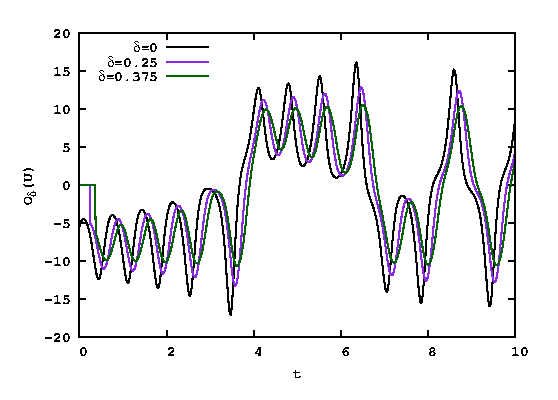
\includegraphics[height=0.5\textwidth]{d025meas.eps}}
\end{figure}

We compute $u$ using equations (\ref{noerra})
with $\widetilde{\cal R}={\cal R}=R_\delta$ 
and $u_0=(0,0,0)$ for different values 
of $\delta$ with $\mu=30$.  
This value of $\mu$ is comparable
to the value $\mu=K/40\approx 38.5$ used for Figure 5 
of \cite{Stuart14}. 
Figure~$\ref{measd}$ illustrates the 
phase shift that occurs for $\delta >0$ which delays the measurements of $U$ in time.

\begin{figure}[ht]\label{avgd}
    \centerline{\begin{minipage}[t]{0.9\textwidth}
    \caption{\label{e0assim}%
	Results when coupling time-averaged exact measurements
	with an averaging window of size $\delta$ when $\delta=\hat\delta$.}
    \end{minipage}}
	\medskip
    \centerline{\includegraphics[height=0.5\textwidth]{e0assim.eps}}
\end{figure}

In particular, Figure~\ref{e0assim} shows the evolution of 
the error $\|U-u\|^2$ when coupling the free-running solution to the
driven solution using noise-free time averaged measurements of $X$
with $\mu=30$ when $\hat\delta=\delta$ for $\delta\in \{ 0, 0.25, 0.375 \}$.
For $\delta=0$ and $\delta=0.25$ the error converges 
to zero within the limits of the floating point arithmetic
used for the computations.
We point out, however, that the rate of convergence
appears slightly slower when $\delta=0.25$.
On the other hand the error remains large for $\delta=0.375$.

\begin{figure}[ht]
    \centerline{\begin{minipage}[t]{0.9\textwidth}
    \caption{\label{avgdup}%
	Results when coupling time-averaged exact measurements
	with an averaging window of size $\delta$ near
$\delta_c$ for $T<2000$ when $\hat\delta=\delta$.}
    \end{minipage}}
	\medskip
    \centerline{\includegraphics[height=0.5\textwidth]{e0assimupper.eps}}
\end{figure}

Further computations show that the conditions for convergence
are intractable when $\delta \approx 0.33$. 
Intuitively, we suspect there is a value $\delta_c$ such that
for $\delta < \delta_c$ the rate of convergence is very slow, but
synchronization is eventually achieved and the error decays to zero,
and for $\delta > \delta_c$ the systems fail to synchronize.
Our calculations suggest $\delta_c\in [0.31,0.33]$, provided such
a critical value exists.
What we do know, is that numerically for values $\delta>0.33$ there
is no sign of synchronization, and for values $\delta<0.31$ the
two solutions synchronize to within the limits of the rounding error
of the double precision arithmetic used for our calculations.
Figure~\ref{avgdup} shows instability of the synchronization
for $\delta = 0.318$, where the error $\|U-u\|^2$ 
oscillates over time through $20$ decimal orders of magnitude.

\begin{figure}[ht]
    \centerline{\begin{minipage}[t]{0.9\textwidth}
    \caption{\label{avgdiffmu}
	Results when coupling time-averaged exact measurements
	with an averaging window of size $\delta = 0.334$ using
    increasing values of $\mu$ where $T<600$ when $\hat\delta=\delta$.}
    \end{minipage}}
	\medskip
    \centerline{\includegraphics[height=0.5\textwidth]{e0diffmu.eps}}
\end{figure}

While the theory requires $\mu$ to be greater than $375.07$,
a slightly less restrictive bound on $\mu$ may be obtained 
by using the value for $K$ suggested by the bound (\ref{numbound}).
Either bound, however, is significantly more restrictive 
than the value chosen here which 
works when the size of the averaging window is sufficiently small.
In this case where $\delta > 0.33$, there are no 
values of $\mu$ for which the error converges to zero, illustrated in
Figure~\ref{avgdiffmu}.

By further varying the value of $\delta$ it appears that
$\delta\le 0.31$ is sufficient to ensure
$\|U-u\|\to 0$ numerically as $t\to\infty$.
We further compare the theoretical size of $\delta$ to 
this numerically determined value.
To find the largest value of $\delta$ that Proposition~\ref{NLTAprop} 
guarantees will lead to synchronization
we maximize the upper bound in 
(\ref{deltabound32}) with respect to $\alpha$.
Note that as $\alpha$ vanishes in the bound (\ref{deltabound32}) 
the length $\delta$ of the time averaging window also 
vanishes.  Moreover, $\delta$ also vanishes as 
$\alpha$ approaches 2,
because $\delta$ depends inversely on $\mu^{3/2}$ and
$\mu$ approaches infinity as $\alpha$ approaches $2$.
Simple
calculus now yields the optimal value of $\alpha$ to be
$$
  \alpha^*=-\rho\cos(\phi)+{22\over 15}+\rho\sqrt3\sin\phi
      \approx 0.28413
$$
where
$$
  \rho={4\sqrt{25370}\over 75}
\wwords{and}
  \phi={1\over 3}\arctan\Big({19\sqrt{1731443695}\over167665}\Big).
$$
For $\alpha=\alpha^*$ it follows that we may take
$$
  \mu\approx 513.153\wwords{and}\delta\approx 0.0000063216.
$$
Using the value for $K$ suggested by the bound 
(\ref{numbound}) leads to a 30 percent larger value for $\delta$;
however, in either case the analytic bounds are more than $10\,000$
times stricter than what works numerically.

In summary our numeric results show
measurements of $X$ averaged with respect to a small
averaging window are just as effective for synchronizing the
driven solution to the free-running solution as exact
measurements taken instantaneously in time.  However, if
the averaging window is too large, then the information is
blurred too much for $u$ to synchronize with $U$.
This is consistent with the theoretical results of
Proposition~\ref{NLTAprop} which proves the
convergence of the driven solution to the free-running
solution only when $\delta$ is sufficiently small and $\mu$
sufficiently large.
We emphasize that our analytic bounds on $\mu$ and $\delta$
are much more restrictive than what works numerically.

\begin{figure}[ht]
    \centerline{\begin{minipage}[t]{0.9\textwidth}
    \caption{\label{avgddhat}%
	Results when coupling time-averaged exact measurements with
    window size $\hat\delta=0.25$ using a feedback term with
	averaging window size $\delta\ne\hat\delta$.  Note that
	$\Delta\delta=\delta-\hat\delta$.
	}
    \end{minipage}}
	\medskip
    \centerline{\includegraphics[height=0.5\textwidth]{mix3a.eps}}
    \centerline{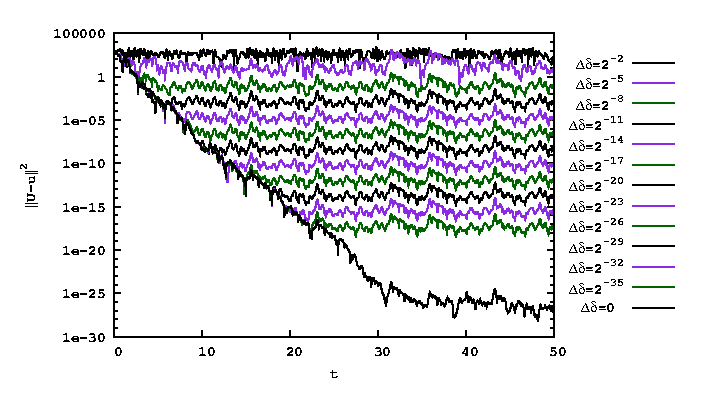
\includegraphics[height=0.5\textwidth]{mix3b.eps}}
\end{figure}

Now consider the case treated by Proposition~\ref{UKNLTAprop} 
where the exact size of the time averaging 
window present in the observational measurements is unknown.
Figure~\ref{avgddhat} describes the evolution of $\|U-u\|^2$ 
when $\hat\delta=0.25$ and $\delta$ is smaller but near 
$\hat\delta$.
Note that $\delta$ greater than
$\hat\delta$ results in a nearly identical graph.
The asymptotic error
%$$\limsup_{t\to\infty} \|U-u\|^2$$
may be approximated numerically as a function of 
$\Delta\delta=\delta-\hat\delta$ by
$$
%	\limsup_{t\to\infty} \|U-u\|^2
%		\approx 
	E(\Delta\delta)=
	\max \big\{\, \|U-u\|^2 : t\in [50,100]\,\big\}.
$$
From Figure~$\ref{avgddhat}$, there is a decrease in the error $\|U-u\|^2$ as
$\Delta\delta$ decreases before reaching $\Delta\delta=0$. 
Table~\ref{tableddhat} illustrates the the convergence of the driven solution, where
the limit supremum is taken over the error for all $t>T$.
As expected, the error levels 
decrease as $\delta$ gets closer to $\hat\delta$.
It is reasonable to determine that there exists a function that will 
allow us to predict
the largest value $|\delta -\hat{\delta}|$ that results in convergence.
We now consider the functional dependency how 
$E(\Delta\delta)$ depends on $\Delta\delta$.


    \begin{table}[h!]\label{tableddhat}
    \centerline{\begin{minipage}[t]{0.9\textwidth}
    \caption{\label{limsupexact}%
	Limsup of $\| U - u\|^2$ for different values of $\Delta\delta$.
    }
    \end{minipage}}
    \medskip
    \centering
    \begin{tabular}{  r | r }
    \hline\hline
\vphantom{\raise8pt\hbox{H}}%
	$\Delta\delta$ & $\limsup \|U-u\|^2$ \\ [0.5ex]
    \hline
\vphantom{\raise8pt\hbox{H}}%
$-2^{-2}$&$1267.31$ \\
$-2^{-5}$&$194.081$ \\
$-2^{-8}$&$5.61624$ \\
$-2^{-11}$&$0.0906275$ \\
$-2^{-14}$&$0.00140762$ \\
$-2^{-17}$&$2.19772\times 10^{-05}$ \\
$-2^{-20}$&$3.43361\times 10^{-07}$ \\
$-2^{-23}$&$5.36495\times 10^{-09}$ \\
$-2^{-26}$&$8.38272\times 10^{-11}$ \\
$-2^{-29}$&$1.30979\times 10^{-12}$ \\
$-2^{-32}$&$2.04656\times 10^{-14}$ \\
$-2^{-35}$&$3.19773\times 10^{-16}$ \\
$0.0$&$2.67042\times 10^{-25}$ \\
[1ex]
\hline
\end{tabular}\qquad\qquad
    \begin{tabular}{  r | r }
    \hline\hline
\vphantom{\raise8pt\hbox{H}}%
	$\Delta\delta$ & $\limsup \|U-u\|^2$ \\ [0.5ex]
    \hline
\vphantom{\raise8pt\hbox{H}}%
$2^{-2}$&$2663.41$ \\
$2^{-5}$&$249.552$ \\
$2^{-8}$&$5.86352$ \\
$2^{-11}$&$0.0911086$ \\
$2^{-14}$&$0.00143265$ \\
$2^{-17}$&$2.24025\times 10^{-05}$ \\
$2^{-20}$&$3.50073\times 10^{-07}$ \\
$2^{-23}$&$5.46996\times 10^{-09}$ \\
$2^{-26}$&$8.54684\times 10^{-11}$ \\
$2^{-29}$&$1.33543\times 10^{-12}$ \\
$2^{-32}$&$2.08664\times 10^{-14}$ \\
$2^{-35}$&$3.26052\times 10^{-16}$ \\
$0.0$&$2.67042\times 10^{-25}$ \\
[1ex]
\hline
\end{tabular}
\label{regress}
\end{table}

%Empirical evidence allows us to infer that there is an exponential function that will fit the rate of
%convergence in terms of $\Delta\delta$. We find that the numerical data 
%supports our results and provides greater
%detail to the exact coefficients necessary for convergence.
The theoretical bounds given by 
Proposition~\ref{UKNLTAprop} suggest that
$E(\Delta\delta)$ is proportional to 
the square of $\Delta\delta$.
In order to test this hypothesis we performed 
a least squares fit to find $m$ and $s$ such that
$$
	\log E(\Delta\delta) \approx \log m + s \log(\Delta\delta).
$$
Figure~\ref{ftmix} shows that the least squares fit
agrees with $E(\Delta\delta)$ to remarkable precision
over a range of ten decimal orders of magnitude.
Since the fitted value $s=1.99964$ 
is so close to $2$, we presume that the $\Delta\delta$ 
dependency given by our analytic bound is physical
even though the values for $\mu$ and $\delta$
are much more restrictive than numerically needed.

\begin{figure}[ht]
    \centerline{\begin{minipage}[b]{0.9\textwidth}
    \caption{\label{ftmix}%
	The numerical data from Table~\ref{limsupexact}
	when plotted with the least squares fit
	of $m(\Delta\delta)^s$
	given by $m=378647$ and $s=1.99964$.}
    \end{minipage}}
	\medskip
    \centerline{\includegraphics[height=0.5\textwidth]{ftmix.eps}}
\end{figure}

It is worth remarking that the theoretical bound in
Proposition~\ref{UKNLTAprop} actually depends on the 
relative error $\Delta\delta/\hat\delta$ which,
as we have held $\hat\delta=0.25$ constant, is
proportional to the absolute error $\Delta\delta$
in the above computations.
Computations using different values for $\hat\delta$
are a direction for future work described in
Section~\ref{futurehatdelta}.  
Preliminary calculations suggest that a better fit
is obtained for bounds of the form
$$
	E(\Delta\delta) \approx m 
			\Big({\delta-\hat\delta\over
			\delta_c-\hat\delta}\Big)^2
$$
where $\delta_c\approx 0.33$ is the critical 
value of $\delta$ for which synchronization fails detailed
in Figure~\ref{avgdup}.
The numerical dependence of the bound on $\hat\delta$ is 
a point of future work.

\chapter{Coupling with Noise}

In this chapter we examine the synchronization of the free running and driven
solutions with the addition of a time-averaged Brownian motion. By
synchronization we mean that the system driven by noisy observations will converge
to the true solution within a tolerance determined by the level of observational noise.
The expected value $\bf E$ of the convergence is examined as we are only able to
bound the error of the system with some probability for a finite
amount of time, preventing us from forming a generalized proof for pathwise convergence.
In particular, we bound the expected value of the error 
and then use Chebyshev's inequality to find probabilistic 
bounds on the paths.

\section{Noisy Instantaneous-in-Time Coupling}

Consider when the observations of $U$
are noisy and satisfy equation~(\ref{tildecO})
%$$\tilde {\cal O}(U)dt = Xdt + \varepsilon dW_t$$
where $W_t$ is a one-dimensional 
standard Brownian motion.
Thus, the noise present in the observational measurements 
satisfies ${\bf Var}(\varepsilon W_t)= t\varepsilon^2$.
In this case, equation~(\ref{drivenX}) becomes
\begin{equation}\label{dxnoise}
    dx = -\sigma(y-x)dt+\mu(X-x)dt + \varepsilon \mu dW_t.
\end{equation}
Note that the noise present in the observations appears
in equation~(\ref{dxnoise}) multiplied by the factor $\mu$.
Therefore, increasing $\mu$ to strengthen the coupling 
between $U$ and $u$
also amplifies the noise.  

The techniques employed are almost identical to those in \cite{Olson14} 
but have been detailed here to provide a concrete point of reference
for comparing our main results which involve time-averaged measurements.
The results in this section, though slightly sharper,
are similar to those which appear in \cite{Stuart14}. 
As in Section~\ref{NLICoupling}, carefully examining the case 
without time-averages first provides a concrete point of reference 
for comparing our results which involve time-averaged measurements.
\begin{proposition}\label{NIprop} 
Suppose $\delta=0$, $\hat\delta=0$ and $\varepsilon>0$.
Let $\mu>K/4-\sigma$, then
$$\limsup_{t\to\infty}{\bf E}\big[||U-u||^2\big] 
	\le
{\mu^2\varepsilon^2\over 
		\sigma+\mu+1-\sqrt{(\sigma+\mu-1)^2+K}
}$$
\end{proposition}

\begin{proof}
With the addition of the noise, equation~(\ref{NLIddotx})
becomes the stochastic differential equation
$$
d(\yourdelta X) = -(\sigma + \mu)\yourdelta X dt + \sigma\yourdelta Y dt
 - \mu
{\varepsilon} dW_t.
$$
Using Ito's formula and the same estimates as in 
Proposition~\ref{NLIprop} we obtain
$$d{V} + \alpha V dt \le 
    2\mu\varepsilon \yourdelta X d W_t +\mu^2\varepsilon^2 dt.$$
Integrating over the interval $[0,t]$ yields
$$
	V(t)e^{\alpha t}-V(0)\le 
		2\mu\varepsilon\delta \int_0^t e^{\alpha s}\yourdelta X(s) d W_s
		+{\mu^2\varepsilon^2 \over \alpha}\big( e^{\alpha t} -1 \big).
$$
Now, taking expected values obtains
$$
	{\bf E}\big[V(t)\big]\le e^{-\alpha t}{\bf E}\big[V(0)\big]
		+{\mu^2\varepsilon^2 \over \alpha}\big( 1-e^{-\alpha t} \big).
$$
Consequently
$$
	\limsup_{t\to\infty} {\bf E}[V] \le {\mu^2\varepsilon^2\over\alpha}.
$$
Solving for $\alpha$ in equation~(\ref{alphadef}) finishes the proof.
\end{proof}

\section{Noisy Time-averaged Coupling}\label{NTACsec}

In this section we consider the case when
the noisy observations
of $X$ have been averaged in time over a known window of 
size $\hat\delta$.  Thus we take $\delta=\hat\delta$ and
%${\cal R}=\widetilde R_\delta$ 
in equation~(\ref{NLTAUnkSoln}) and
equation~(\ref{drivenX}) becomes
$$
	\dot x = -\sigma(y-x) +\mu(\bar X-\bar x)+\mu\xi
\words{where} \xi(t)={\varepsilon\over\delta}\big(W_t-W_{t-\delta}\big).
$$
Thus
$$
	\yourdelta\dot X 
	=-(\sigma+\mu)\yourdelta X+\sigma\yourdelta Y +
		\mu(\yourdelta X-\yourdelta\bar X)+\mu\xi.
$$
Theoretically the presence of a small time average in the measurements 
does not substantially affect the results of the instantaneous in
time case.
Our results show that measurements averaged over
small time windows lead to bounds that are similar to those given 
by Proposition~\ref{NIprop} when there are no time averages.
The expected value of the difference 
between the driven solution and the free running solution in
both cases is bounded by a constant factor of the variance of the noise.
In particular, we have

\begin{proposition}\label{NTAprop} 
Let $\alpha\in(0,2)$ and $\mu\ge K/(2-\alpha)^2-\sigma$.  If
$$	\delta<
	\sqrt{{1-e^{-1}\over 2}\cdot {\alpha\over 32\mu(\sigma+\mu)^2}}.
$$
Then
$$
	\limsup_{t\to\infty} {\bf E}\big[\|U-u\|^2\big] <
	e\Big({8\mu^3\over\alpha^2}+{2\mu\over \alpha^2\delta}\Big)
		\varepsilon^2.
$$
\end{proposition}

\begin{proof} 
The proof proceeds as the proof of Proposition~\ref{NTAprop}, where the
only difference is an additional noise term.
Similar estimates as in the proofs of Lemma~\ref{tadiffit}
and Lemma~\ref{tadiffithat} yield that
$$
	|\Delta X-\Delta\bar X|^2
		\le
		4\delta(\sigma+\mu)^2
		\int_{t-2\delta}^t \big\{|\Delta X|^2+|\Delta Y|^2\big\}
		+4\mu^2\delta\int_{t-\delta}^t\xi^2.
$$
Following similar estimates as before, multiply 
by $\yourdelta X$ and use Young's inequality as
\begin{plain}$$\eqalign{
    \mu(\yourdelta X - \yourdelta\bar{X})\yourdelta X
		&\le
    	{4\delta\mu (\sigma + \mu)^2\over \alpha}
		\int_{t-2\delta}^t 
		\big\{|\yourdelta X|^2 + |\yourdelta Y|^2\big\}\cr
		&\qquad
		+{4\mu^3\delta\over \alpha}\int_{t-\delta}^t\xi^2
+{\alpha\mu\over 4}|\yourdelta X|^2
}$$\end{plain}%
and
\begin{plain}$$\eqalign{
\mu\xi \yourdelta X
&\le 
 {\mu\xi^2 \over
    \alpha}+
{\alpha\mu \over 4} |\yourdelta X|^2 .
}$$\end{plain}
to obtain
$$
    \dot{V} + \alpha V
    \le {8\delta\mu(\sigma + \mu)^2 \over \alpha}
	\displaystyle\int_{t-2\delta}^t(\yourdelta X^2 +
    \yourdelta Y^2) 
	+{8\mu^3\delta\over\alpha} \int_{t-\delta}^t \xi^2
	+{2\mu\xi^2 \over \alpha}.
$$
Since ${\bf E}[\xi^2]=\varepsilon^2/\delta$ for any time $t$, 
then setting
$\cV(\tau)={\bf E}[V(\tau/\alpha)]$ yields
$$
{d{\cV}(\tau)\over d\tau} + \cV(\tau) \leq 
	{8\delta\mu(\sigma + \mu)^2\over \alpha^3}
		\int_{t-2\alpha\delta}^t \cV(s)\,ds
+\Big({8\mu^3\over\alpha^2}+{2\mu \over \alpha^2\delta}\Big)\varepsilon^2.
$$
We apply Lemma~\ref{intGronwallerror} 
taking 
$$A=
	{8\delta\mu(\sigma + \mu)^2\over \alpha^3},\qquad
B=
\Big({8\mu^3\over\alpha^2}+{2\mu \over \alpha^2\delta}\Big)\varepsilon^2
\qquad\hbox{and}\qquad h=2\alpha\delta.$$
The result follows.
\end{proof}

\section{Unknown Noisy Time-averaged Coupling}\label{UNTACsec}

In this section we examine the case when there is noise in
the measurements and the length of the time averaging window 
is unknown.  
Our main result is a version of Proposition~\ref{UKNLTAprop}
that also allows noise in the observations.
As before let $\hat\delta$ be the length of the unknown averaging
window in the observations of the free running solution and
$\delta$ be an approximation of $\hat\delta$ that will be used 
in the feedback control of the driven system.
In this case the equation governing the evolution $x$ in the driven system
becomes
$$
    \dot{x} = -\sigma(y-x)+\mu
        \Big(
        {1\over\hat\delta}\int_{t-\hat\delta}^t X(s)ds
        -{1\over\delta}\int_{t-\delta}^t x(s)ds
    \Big) + \mu\xi
$$
where $\xi$ is as in Section~\ref{NTACsec}.
Since there is now noise in the observations, exact synchronization does 
not occur when $\delta=\hat\delta$.  Thus, our theoretical bounds
on $\|U-u\|^2$ take the form given by equation~(\ref{noisydeltadelta}) consisting
of two terms, one which vanishes as $\delta\to\hat\delta$ and
the other which vanishes as $\varepsilon\to 0$.
In particular, we obtain

\begin{proposition}\label{UKNTAprop}
Suppose $\delta\ne\hat\delta$ and $\varepsilon>0$.
Given $\alpha\in(0,2)$,
let 
$$\mu \ge JK/(2-\alpha)^2-\sigma
\words{where}
		J={\sigma(1+\sqrt 2)}
        \Big({\hat\delta\over 2} +\delta\Big)+1.
$$ 
and 
$$  \delta<
    \sqrt{{1-e^{-1}\over 2}\cdot {\alpha\over 32\mu(\sigma+\mu)^2}}.$$
Then $$\limsup_{t\to\infty}{\bf E}\big[\|U-u\|^2 \big]
< {5e(2-\alpha)\mu^2\over \alpha}\cdot
{(\hat\delta-\delta)^2\over\hat{\delta}^2}
	+
    e\Big({16\mu^3\over\alpha^2} +{2\mu\over\alpha^2\hat\delta}\Big)\varepsilon^2.
$$
\end{proposition}

\begin{proof}
Modifying the proof of Lemma~\ref{tadiffithat}
we add the term for measurement error, which yields
\begin{align*}
	|\Delta X-\Delta\bar X|^2
		&\le
		4\delta(\sigma+\mu)^2
		\int_{t-2\delta}^t \big\{|\Delta X|^2+|\Delta Y|^2\big\}\\
		&+16 \mu^2\delta^2 K \Big({\delta-\hat\delta\over\hat\delta}\Big)^2
		+8\mu^2\delta\int_{t-\delta}^t\xi^2.
\end{align*}
Now, modifying the proof of Proposition~\ref{UKNLTAprop} as was done
for the proof of Proposition~\ref{NTAprop} to add the term which
represents measurement error yields 
\begin{align*}
    {d\cV(\tau)\over d\tau}
+ \cV(\tau)
    &\leq
        {8\delta\mu (\sigma + \mu)^2\over \alpha^3}
        \int_{\tau-2\alpha\delta}^\tau \cV(s)\,ds\\
		&+16 \mu^2\delta^2 K \Big({\delta-\hat\delta\over\hat\delta}\Big)^2
			+{2\mu\over\alpha\eta} 
            +{16\mu^3 \over \alpha^2}
	+ {2\mu\varepsilon^2\over \alpha^2\delta}.
\end{align*}
Applying Lemma~\ref{intGronwallerror} 
finishes the proof.
\end{proof}


\section{Numeric Results for Noisy Coupling}\label{NoisyComp}

The first set computations in this section treat the case 
where no time averaging is present in the observational measurements.
Under this hypothesis Proposition~\ref{NIprop} 
shows that the expected value of the difference between 
the approximating solution and the exact solution
is bounded by a factor of the variance of the noise.
A similar bound was obtained 
%by Law, Shukla and Stuart 
as Theorem 4.1 
in \cite{Stuart14} which, using the notation here, may be written as
\begin{equation}\label{stubound}
	\limsup_{t\to\infty} {\bf E}\big[\|U-u\|^2\big] \le 
	{\mu^2\varepsilon^2\over 2-K/(2\mu)}
\qquad\hbox{for}\qquad \mu>K/4.
\end{equation}
Optimizing the bound in the bound (\ref{stubound}) with respect to $\mu$ and 
using the value of $K$ given by Theorem~\ref{Ktheorem}
we obtain that 
$$
	\limsup_{t\to\infty} {\bf E}\big[\|U-u\|^2\big] \le 
	{27K^2\varepsilon^2\over 128}\le (5.005\times 10^5)\varepsilon^2.
$$
Alternatively, 
optimizing the bound in Proposition~\ref{NIprop} yields
$$
	\limsup_{t\to\infty} {\bf E}\big[\|U-u\|^2\big] \le 
	(4.838\times 10^5) {\varepsilon^2}
$$
which is about 3 percent smaller.  
Moreover, since
$$
{\mu^2\varepsilon^2\over 
		\sigma+\mu+1-\sqrt{(\sigma+\mu-1)^2+K}}
<{\mu^2\varepsilon^2\over 2-K/(2\mu)}
$$
provided $\mu>K/4$, the bound given in the bound (\ref{stubound}) is
strict.  Therefore, there exists $T>0$ such that
by Chebyshev's inequality 
$$
	{\bf P}\Big\{\,\omega\in\Omega : \|U-u\|^2\le 
{10\mu^2\varepsilon^2\over 2-K/(2\mu)}
\,\Big\}
		\ge 0.9.
$$
Computations in \cite{Stuart14} demonstrate
numerical bounds on $\|U-u\|$ which are proportional to 
$\varepsilon$ and therefore consistent with
the theoretical bounds described above.
In the present thesis we fix the noise level at 
$\varepsilon=0.01$ and focus on the effects of the 
time averaging.

\begin{figure}[ht]
    \centerline{\begin{minipage}[b]{0.9\textwidth}
    \caption{\label{e001paths}%
	Results when coupling noisy instantaneous-in-time measurements
	with $\mu=30$ and $\varepsilon=0.01$. The expected value was 
	computed using 500 independent realizations of Brownian motion
	and $L(t)$ is a computed bound on $90$ percent of the paths at 
	each point in time.
	The gray region represents the 500 pathwise solutions, one of which
    has been plotted in a darker shade for illustration.}
	\medskip
    \end{minipage}}
    \centerline{\includegraphics[height=0.5\textwidth]{e001paths.eps}}
\end{figure}

For a frame of reference, first consider 500 independent
realizations of Brownian motion corresponding to 
$\omega_i\in\Omega$ such that $i=1,2,\ldots,500$ and 
compute the corresponding pathwise solutions $u_i$ using 
equation~(\ref{noerra}) with the coupling 
term ${\cal R}=\widetilde R$.
The exact algorithm used to compute $u$ shall 
be described later in Section~\ref{numerics}.
Approximate the expected value of $\|U-u\|^2$ by
$$
	{\bf E}\big[\|U-u\|^2\big]\approx
		{1\over 500} \sum_{i=1}^{500} \|U-u_i\|^2
$$
and let $L(t)$ be the value such that
$$
	{\rm card}\big\{\, i\in \{1,2,\ldots,500\} 
		: \|U-u_i\|^2\le L(t)\,\big\} = 450.
$$
Thus, $L(t)$ bounds $90$ percent of the
paths at each point in time.
In particular, assuming $500$ samples is statistically large enough, 
we have
$$
	{\bf P}\big\{\,\omega\in\Omega : \|U-u\|^2\le L(t)
		\,\big\} \approx 0.9.
$$
Figure~\ref{e001paths} describes
the results of this first computation.  Note that the
expected value of 
$\|U-u\|^2$ oscillates around $0.01$ and
that $L(t)$ is about 5 times greater.
Thus, $L(t)$ is about 2 times smaller than the bound
given by Chebyshev's inequality (\ref{cheby}).
Moreover, at each point in time a small percentage 
of trajectories are significantly more accurate than
expected and a few satisfy $\|U-u_i\|^2\le\varepsilon^2$.

The computation described in Figure~\ref{e001paths} may
be directly compared to Figure 5 in \cite{Stuart14}.
Similar values of $\mu$ and $\varepsilon$ were employed
in both computations and result in similar looking
pathwise solutions.  The difference is that our
expected values have been computed by averaging
over the pathwise solutions $u_i$ which result from 
independent Brownian motions and approximate
the time-dependent expected values which appear in 
the analysis,
whereas~\cite{Stuart14} computes expected values that 
do not change over time and appear to have been computed 
by taking a long-time average over a single pathwise solution.
We now consider how the presence of time averaging in the
observational measurements affects the degree to which 
$u$ synchronizes with~$U$.

\begin{figure}[ht]
    \centerline{\begin{minipage}[b]{0.9\textwidth}
    \caption{\label{e001meas}%
	Time-averaged noisy measurements 
	for different values of $\delta$ corresponding to a 
	representative Brownian path
    with $\varepsilon=0.01$.}
	\medskip
    \end{minipage}}
    \centerline{\includegraphics[height=0.5\textwidth]{e001mtalk.eps}}
\end{figure}

Figure~\ref{e001meas} depicts the time evolution of a typical 
set of noisy observational measurements with and without time 
averaging.
Note that when $\hat\delta=0$ there is no time
averaging and resulting observations show
oscillation of the trajectory,
As we are dealing with a chaotic system, we can expect that these oscillations
will perturb the system enough so that synchronization is only possible within
a tolerance of the measure of the noise.
When $\hat\delta>0$
the noise has been smoothed out at the expense of a phase
shift that delays the measurements in time.  We now perform
a number of calculations of $u$ using measurements of
the kind depicted in Figure~\ref{e001meas}.

Figure~\ref{e001exp} depicts the evolution of the expected
value of $\|U-u\|^2$ over time for $\mu=30$,
$\varepsilon=0.01$ and $\delta\in \{ 0, 0.25, 0.375 \}$.
As in the noise-free case, the difference between $u$ and $U$ 
remains large when $\delta=0.375$.
However, the difference between $\delta=0.25$ and $\delta=0$
appears greater than in the noise-free case.
Intuitively, the presence of moving time averages seems to 
result in decreased efficiency of the feedback control 
that nudges the driven solution towards the free running solution.
Without noise, only enough nudging to overcome the tendency for 
nearby trajectories of the Lorenz equation to diverge is needed.
As the nudging must also overcome the noise in the present case,
which in turn may account for the expected error levels being 
slightly greater when $\delta=0.25$.
Further support for this intuition may also be inferred from 
the already mentioned slower rate of convergence in the absence of noise 
$\delta=0.25$ compared to $\delta=0$.

\begin{figure}[ht]
    \centerline{\begin{minipage}[b]{0.9\textwidth}
    \caption{\label{e001exp}%
	Results when coupling time-averaged 
	noisy measurements with an
	averaging window of size $\delta$ and
a noise level $\varepsilon=0.01$.
	The expected values were computed using 500 independent
	realizations of Brownian motion.}
    \end{minipage}}
	\medskip
    \centerline{\includegraphics[height=0.5\textwidth]{e001exp.eps}}
\end{figure}

\begin{figure}[ht]\label{mixassim}\label{mix3ae001}
    \centerline{\begin{minipage}[b]{0.9\textwidth}
    \caption{\label{mix3a}%
    Results when coupling time-averaged noisy measurements with
	$\varepsilon=0.01$ and
    window size $\hat\delta=0.25$ using a feedback term with
    averaging window size $\delta\ne\hat\delta$.  Note that
    $\mu=30$ and $\Delta\delta=\delta-\hat\delta$.
    }
    \end{minipage}}
    \medskip
    \centerline{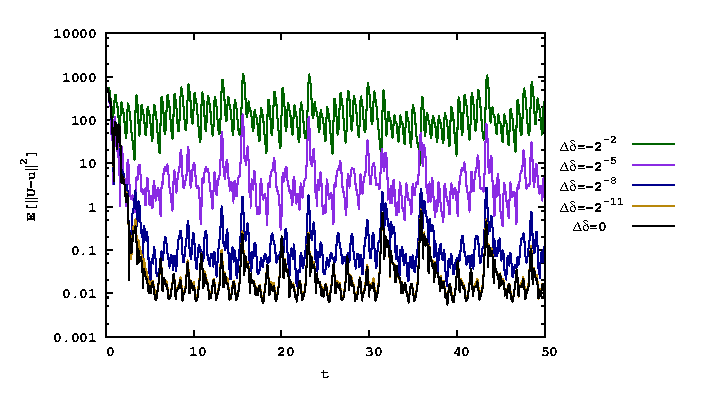
\includegraphics[height=0.5\textwidth]{mix3ae001.eps}}
    \centerline{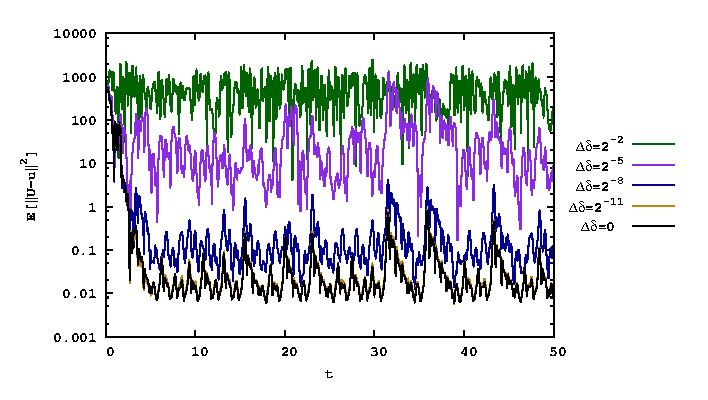
\includegraphics[height=0.5\textwidth]{mix3be001.eps}}
\end{figure}

Figure~\ref{e001exp} depicts the evolution over time of
the expected value of $\|U-u\|^2$ for $\mu=30$,
$\varepsilon=0.01$ and $\delta\in \{ 0, 0.25, 0.375 \}$ with
respect to
500 independent realizations of noisy measurements of the kind
depicted in Figure~\ref{e001meas}.
As in the noiseless case, the difference between $u$ and $U$
remains large when $\delta=0.375$.
Similarly, for $\delta=0.25$ and $\delta=0$ the error decreases
over time; however, unlike the noiseless case
the asymptotic error level for $\delta=0.25$ is
noticeably larger than for $\delta=0$.  In particular,
\vfill\eject
\begin{plain}$$
\max\big\{\,{\bf E}\big[\|U-u\|\big]:t\in[50,100]\,\big\}\approx
\cases{
    0.0089 & for $\delta=0$\cr
    0.49 & for $\delta=0.25$.
}
$$\end{plain}%

Intuitively, the presence of moving time averages seems to
result in a decreased efficiency of the feedback control
that nudges the driven solution towards the free running solution.
Without noise, this decrease in efficiency doesn't matter
because the difference between the free running and driven
solutions tends to zero over time anyway, only perhaps
with a slightly decreased rate of convergence.
In the presence of noise, however, the nudging must also
overcome the noise.
This leads to a higher error level in the difference
between $U$ and $u$ over time.

The last set of computations treats the case in
Proposition~\ref{UKNTAprop} when the length of
the averaging window used for the observations is unknown.
Figure~\ref{mix3ae001} depicts the evolution
of the expected value of $\|U-u\|^2$ when
$\hat\delta=0.25$ and $\delta$ is smaller but near $\hat\delta$.
The error level decreases as
$\delta$ gets closer to $\hat\delta$, but unlike the noiseless
case, there is very little difference between
$\Delta\delta=0$ and $\Delta\delta=-2^{-11}$.
Bounds on the expected error may be approximated
numerically as
$$
    \widetilde E(\Delta\delta)
    =\max\big\{\, {\bf E}\big[\|U-u\|^2\big] :
        t\in[50,100]\,\big\}.
$$
A summary of our computations are presented in
Table~\ref{limsupe001}.
These numeric results show, as do our theoretical bounds,
that $\delta$ can be tuned to match $\hat\delta$ only up to
the point where the noise term dominates.
Specifically,
when $\hat\delta=0.25$ and $\epsilon=0.01$
%our computations suggest
it is possible
to tune $\delta$ so that $|\delta-\hat\delta|< 2^{-8}$.

As seen in Figure~\ref{e001meas} typical values of $X$
range from $-10$ to $10$.  Moreover, the free running
solution used in our experiments satisfies
$$
    \Big({1\over 100}\int_0^{100} X(s)^2ds\Big)^{1/2}
        \approx 7.92731.
$$
We finish by noting that $\varepsilon=0.01$ is $1.3$
percent the root-mean-squared value of $X$ and that
$2^{-8}$ is $1.6$ percent the value of $\hat\delta$.
The exact relationship between the value of $\varepsilon$
and the degree to which $\delta$ can and needs to be tuned
would be an interesting direction for future study.

\begin{table}[ht]
    \centerline{\begin{minipage}[b]{0.9\textwidth}
    \caption{\label{limsupe001}%
    Values of
    $\widetilde E(\Delta\delta)=
    \max \big\{\, {\bf E}\big[\|U-u\|^2\big] : t\in [50,100]\,\big\}$
    as a function of $\Delta\delta=\delta-\hat\delta$.
    Here $\hat\delta$ represents
    the unknown size of the averaging present in the observational
    measurements and
    $\delta$ an approximation of $\hat\delta$ used in the feedback
    control.}
    \end{minipage}}
    \bigskip
    \centering
    \begin{tabular}{  r | r }
    \hline\hline
\vphantom{\raise8pt\hbox{H}}%
%   $\Delta\delta$ & $\limsup \|U-u\|^2$ \\ [0.5ex]
    $\Delta\delta$ & $\widetilde E(\Delta\delta)$ \\ [0.5ex]
    \hline
\vphantom{\raise8pt\hbox{H}}%
$-2^{-2}$&$1.60729\times 10^{6}$ \\
$-2^{-5}$&$38419.5$ \\
$-2^{-8}$&$44.133$ \\
$-2^{-11}$&$0.693591$ \\
$0$&$0.491966$ \\
[1ex]
\hline
\end{tabular}\qquad\qquad
    \begin{tabular}{  r | r }
    \hline\hline
\vphantom{\raise8pt\hbox{H}}%
%   $\Delta\delta$ & $\limsup \|U-u\|^2$ \\ [0.5ex]
    $\Delta\delta$ & $\widetilde E(\Delta\delta)$ \\ [0.5ex]
    \hline
\vphantom{\raise8pt\hbox{H}}%
$2^{-2}$&$6.09399\times 10^{6}$ \\
$2^{-5}$&$62104.1$ \\
$2^{-8}$&$38.5955$ \\
$2^{-11}$&$0.56483$ \\
$0$&$0.491966$ \\
[1ex]
\hline
\end{tabular}
\end{table}

\chapter{Numerical Methods}\label{numerics}

This section described the numerical methods used to obtain the 
results in Section~\ref{NoiselessComp} and Section~\ref{NoisyComp}.
We compute both the free running solution and the driven solution
using Euler's explicit method
\begin{plain}$$\eqalign{
	U^{n+1}&=U^{n}+h{\cal F}(U^n)\cr
	u^{n+1}&=u^{n}+h{\cal F}(u^n)+
		h\mu\big(R_{\hat\delta}(U^n)-R_\delta(u^n)\big)
		+h\mu\hat\xi^n
.\cr
}$$\end{plain}%
in double-precision floating-point arithmetic
with step size $h=1/2048$. 
Here $\hat\delta=m_0h$ for some $m_0\in{\bf N}$
but $\delta$ may be any positive floating-point number.
Upon writing $U^n=(X_n,Y_n,Z_n)$ and $u^n=(x_n,y_n,z_n)$, it 
follows that $R_\delta={\cal L}\circ{\cal O}_{\delta}$ where
$$
	{\cal O}_{\hat\delta}(U^n)={1\over m_0}\sum_{k=0}^{m_0-1} X_{n-k}
$$
and 
by interpolation 
setting $m_3=\lfloor\delta/h\rfloor$ that
$$
	{\cal O}_{\delta}(u^n)=
	{h\over\delta}\Big\{
		\Big({\delta\over h}-m_3\Big)
		x_{n-m_3}+
			\sum_{k=0}^{m_3-1} x_{n-k}
		\Big\}.
$$

%\chapter{Standard Brownian Motion}

The noise term $\hat\xi^n=\hat\xi(nh)$ is given as in Section~\ref{UNTACsec}
by
$$
	\hat\xi(t)={\varepsilon\over\hat\delta}\big(W(t)-W(t-\hat\delta)\big)
$$
where $W(t)$ is a standard Brownian motion,
one of the simplest of the continuous-time stochastic 
processes.
Numerically we use the construction of Brownian
motion as developed by L\'evy and Ciesielski.
By L\'evy and Ciesielski, there is a probability space $\Omega$ and a sequence
of independently distributed standard normal random variables $(G_n)_{n\ge 0}$
such that for $\omega\in\Omega$ and $t\in[0,1]$
$$
W(\omega, t)= \lim_{n\to\infty} W_n(\omega,t)
\wwords{where}
	W_n(\omega,t)=\displaystyle\sum_{k=0}^n G_k(\omega)S_k(t)
$$
is a Brownian motion, where $S_n(t)$ is from the family of Schauder functions.
The Schauder functions $S_{2^j+k}$ are tent-functions with support $[k2^{-j},
(k+1)2^{-j}]$ and a maximal value $\textstyle{1\over 2}2^{-j/2}$ at the tip of the
tent.
Using an application of Minkowski's inequality, monotone convergence theorem,
and by the completeness of the space of continuous functions, there is a
subsequence of $(W_{2^j}(t, \omega))_{j\ge 1}$ which converges uniformly in
$t\in[0,1]$ for a subset $\Omega_0\subset \Omega$.
Defining $W(t, \omega)$ as a limiting function, we see that it
indeed inherits the continuity of $W_{2^j}(t, \omega)$. We conclude that there
exists a restriction of $W(t, \omega)$ that is a Brownian motion defined on
$\Omega$.

The algorithm for the construction of Brownian motion is an adaptation based on
L\'evy's original interpolation argument.
Let $t_0<t<t_1$ and let $W(t)$ be a Brownian motion. Then,
$$ 
G' = W(t) - W(t_0) \wwords{and} G'' = W(t_1) - W(t)
$$ 
are Gaussian random variables with mean zero and variances $t-t_0$ and $t_1-t$
respectively. Let $\Gamma$ be a further $N(0,1)$ random variable which is
independent of $W(t_0)$ and $W(t_1) - W(t_0)$. 
If $t$ is the midpoint of $[t_0,
t_1]$, then $\Gamma$ is a random variable with the same distribution as
$W(t)$ and is a one-dimensional Brownian motion. 
\begin{theorem}\label{levy}(Levy 1940)
    The series 
    $$
    W(t, \omega) = \displaystyle\sum_{n=0}^\infty \big(W_{2^{n+1}}(t,\omega) -
    W_{2^{n}}(t, \omega)\big) + W_1(t,\omega), \qquad t\in[0,1]
    $$
    converges a.s. uniformly. In particular, $\big(W(t)\big)_{t\in[0,1]}$ is a
    Brownian motion.
\end{theorem}
$W(t)$ is almost surely continuous and can be constructed
iteratively using independent increments.
This algorithm is based on L\'evy's construction of Brownian motion
by means of a limit as $n\to\infty$ of piecewise linear functions 
taken on subsequently finer and finer refinements of a dyadic grid
of size $1/2^n$.
Numerically, continuous time processes are sampled 
on a finite grid as we can only generate finitely many values in
finite time.
Assuming we have already constructed $W(k2^{-j})$ for some fixed $j\ge 1$ and all $k \in [0,2^j]$, 
then
$$
    W(l2^{-j-1}) = \begin{cases}
                        W(k2^{-j}) \qquad &l = 2k\\
                        \textstyle{1\over 2}(W(k2^{-j}) +
                        W((k+1)2^{-j})) + \Gamma_{2^j +k} \qquad &l = 2k+1\\
                   \end{cases}
$$
so $W_{2^j}(t)$ is therefore a piecewise linear interpolation of the Brownian path
$W(t)$.
We take the size of the time steps used in our
numerical simulations equal to $h=1/2^n$ so that no further 
processing is needed to compute $W(t)$ at the values needed
for our numerical simulations.
This results in a numerical approximation of Brownian motion,
where any refinement of the discretization yields a refinement of the
same simulated path.  The points on the discrete time grid are simulated
linearly, which is possible as Brownian motion has continuous paths.

The seed of the random generator provides a unique random
variable $\omega$ in the Gaussian space $\Omega$ used to create a unique Brownian motion.
The refinement of an already simulated path
is an interpolation in $[t_0, t_1]$
taken as dyadic points $t= k2^{-j}$ the expansion of $W(t, \omega)$ is finite and
we are able to calculate the value of
$W(t, \omega)$, by successive approximations $t \to W(t, \omega)$.
Set $W(0,\omega)$ to zero and let $W(1,\omega)$ be an $N(0,1)$ 
distributed random variable.
The initialization of $\omega \in \Omega$ as an $N(0,1)$ distributed random
variable is implemented using 1024-bit Marsaglia pseudo-random 
number generators \cite{Marsaglia2003}.
The random numbers generator may take a fixed seed as an input, and as such,
the same Brownian 
path can be sampled at any resolution on the dyadic grid. In this way we were able
to change the time-scale of the simulation without changing the results from
previous experiments.
We initialize the L\'evy-Ciesielski algorithm with an initial refinement, then refine
as needed to support our averaging scheme. The algorithm as described in
the chapter on simulation by Bj\"orn B\"ottcher in
Schilling and Partzsch \cite{Schilling2012},
can be described as follows,

\begin{algorithm}[ht]
 \textbf{Algorithm:} (L\'evy-Ciesielski)\\
Let $J\ge1$ we the order of refinement.\\
Initialize $w_0 := 0$\\
Generate $w_1 \sim N(0,1)$\\
 \For{$j=0$ to $J-1$}{
    \For{$l= 0$ to $2^j - 1$}{
    1. Generate $y \sim N(0,1)$\\
    2. Set $w_{(2l+1)/2^{j+1}} = \textstyle{1\over 2}(w_{l/2^j} + w_{(l+1)/2^j}) 
    + 2^{-(\textstyle{j\over 2} + 1)}y$\\
    }
 }
\textbf{Then} $(w_0, w_{1/2^J}, w_{2/2^J},\cdots , w_1) \sim (W_0, W_{1/2^J}, W_{2/2^J},\cdots , W_1)$
\end{algorithm}

Note that taking $\hat\delta=h$ reduces $\hat\xi^n$
to exactly the term used in the Euler-Maruyama method
for the simulation of the stochastic differential
equation given by equation~(\ref{dxnoise}).  
Thus, taking $\hat\delta=h$ in our computations corresponds 
to noisy in\-stan\-tan\-eous-in-time coupling in our analysis.
Although the sample paths of our Brownian motions 
do not depend on $h$, 
the sensitive dependence of the 
Lorenz system on initial conditions and the 
resulting deterministic chaos exhibited implies that the 
free running solution $U$ strongly depends on $h$.
Therefore, we have fixed $h=1/2048$ to ensure that the same 
reference solution $U$ is considered in all our simulations.

Theoretically, if $\delta=\hat\delta$, $u_0=U_0$ and $\varepsilon=0$, 
then $u(t)=U(t)$ for all $t\ge 0$ and any value of $\mu$.  
This property is preserved at the discrete level in our numerics.
In particular, when $\delta=\hat\delta$ and $\varepsilon=0$
exact synchronization of $u^n$ with $U^n$ is possible and was 
observed in certain simulations.
Exact bit-for-bit synchronization of $u^n$ with $U^n$ seems to
result from a lucky coincidence in the rounding of the floating 
point arithmetic, whereas, in general synchronization is
only good up to the least significant bits.
Note when $\delta\ne\hat\delta$ or $\varepsilon>0$ that
exact synchronization is neither theoretically possible nor 
was numerically observed.

\chapter{Conclusions}

This thesis considers coupling two systems of equations using
noisy partial observations of the phase space that have been
blurred in time by means of a moving time average.
The inclusion of blur using time averages in the observational 
measurements is both realistic from a physical point of view
as well as tractable in our mathematical and numerical frameworks.
The major contributions of our study are four new theorems 
that cover time averages and numeric simulations that show
the coupling works even better than what is guaranteed by
the analysis.  Namely, the original work in this thesis
centers on the statements and proofs of Propositions \ref{NLTAprop},
\ref{UKNLTAprop}, \ref{NTAprop} and \ref{UKNTAprop} and the
corresponding numeric simulations.

In the context the model system, the Lorenz equations, we have shown that the 
data-assimilation method introduced in \cite{Olson14} is well-posed
when the observational data is contaminated by a moving average
with sufficiently short averaging window. In the noiseless case,
analysis and numeric simulation shows that synchronization
of the driven solution to the free-running solution occurs when
the time averaging window is known and small enough.
Moreover, when the time averaging window is unknown, the bound on 
the error is proportional to $(\Delta\delta)^2$ where $\Delta\delta$ 
is the difference between the size of the actual averaging window 
and the guess for the size of the window used in the feedback
control.

In the presence of noise, time averaging smooths out the noise
in the observational measurements at the expense of a phase
shift that delays the measurements in time.
Although averaging gives no improvement in the analytic and numerical
bounds on $\|U-u\|$, there is also no significant deterioration 
in those bounds provided the averaging window is small enough.
In fact, this is the punch line of this thesis:  {\it short time
averages can be compensated for in the feedback term and as a
result have minimal effect on the quality of the synchronization 
between the free-running solution and the driven solution.}
Note, however, that time averaging appear to slightly weaken the
coupling between the driven and the free-running solution
which, in turn, yields a slight increase in the expected error levels.

\chapter{Future Work}

\section{Improved Bound on Fractal Dimension of Attractor}
	\label{fractalbound}
Using the improved ellipsoid described in Appendix~A, we conjecture that
an improved analytic bound on the fractal dimension of the global
attractor ${\cal A}$ of the Lorenz equations may be found using the
techniques in Doering and Gibbon \cite{Doering95a}.

\section{Numerically Determined Upper Bound}

In the case where the size of the averaging window is unknown, we conjecture
that an improvement to the analytical bound given in 

Noting that in Figure~\ref{mixassim} the difference between ${\bf E}[\| U - u\|^2]$ and $L(t)$ is less than a factor of $2$, it may be possible to compute a bound numerically that will improve the bound obtained analytically using the Chebyshev inequality.
By using a non-linear least squares we postulate that an upper bound on $\| U - u\|$ can be determined in the case where the averaging window of $U$ is unknown.

\section{Adapting $\mu$ by Computing Local Lyapunov Exponents}

We postulate that an improvement on convergence can be achieved through the use
of an adaptive filter that tunes the $\mu$ parameter as the system evolves by
testing the rate of convergence at time $t$.

We conjecture that an adaptive filter may be constructed by computing local
Lyapunov numbers. By determining the rate of divergence of the trajectories, we can allow 
for larger values of $\mu$ when the system is 'well-behaved', 
In the noiseless case, we can achieve synchronization for unstable values of
$\delta$ such as $\delta = 0.318$ as shown in Figure~\ref{avgdup}.
In the noisy case, the noise in the observations can be made
to be smooth enough that convergence below the level of observational noise can be achieved. 

\section{Reconstructing Attractor Dynamics}

Takens' \cite{Takens81} proved that the time-delayed 
versions 
$$
[y(t),y(t-\tau),y(t-2\tau),\cdots,y(t-2n\tau)]
$$ 
of one generic signal would suffice 
to embed the $n$-dimensional manifold. 
This may be compared to the topological result
by Whitney \cite{Whitney36} in which a single observation
in $2n+1$ dimensions can be replaced by $2n+1$ observations
of one dimension.  Namely, Taken's proved

\begin{theorem} Let $M$ be a compact manifold of dimension $d$. 
For pairs $(\phi, h)$,
where $\phi : M \to M$ is a smooth (at least $C^2$) diffeomorphism and 
$h : M \to R$ a smooth
function, it is a generic property that the $(2d +1)$-fold observation map
$H_k[\phi, h] : M \to \R^{2d+1}$
defined by
$$
x \to (h(x), h(\phi(x)), \ldots, h(\phi^{2d} (x)))
$$
is an immersion (i.e. $H_k$ is one-to-one between $M$ and its image with both 
$H_k$ and $H^{-1}_k$ differentiable).
\end{theorem}
The theorem can be applied to time series by taking $\phi$ to be the time $T$ map of
the underlying
(continuous time) dynamical system, i.e. $\phi_j (x_0) = x(jT)$, 
where $x(t·)$ is the
trajectory starting
at $x_0$. 
Since $H_k$ is a diffeomorphism 
its inverse is differentiable) this reconstruction
preserves the
dimension of any invariant set and the Lyapunov exponents of the flow.
\begin{figure}[ht]\label{reconst}
\begin{center}
\caption{Lorenz attractor reconstructed in $X$ with time delay $T = 1$.}
\includegraphics[width=10cm]{lorenz_reconst.eps}
\end{center}\end{figure}

We can see from Figure~$\ref{reconst}$ that the reconstruction of the Lyapunov
attractor results in similar, but not identical geometry in the phase space. 
However, according to Takens' Theorem, the Lyapunov spectrum and the correlation
dimension are preserved by the embedding. It is therefore reasonable to assume
that a system constructed by averages where $\delta < \delta_c$ will also
preserve these properties. In this case he phase space of $U$ will be exactly
the sets of observational data. It will be difficult to compute $H^{-1}$
directly or exactly. Therefore we may be able to compute $H^{-1}$ by
approximating its determining form as defined in \cite{Jolly15}.

\section{Unknown Dynamics of Free Running Solution}
\label{whatissigma}
It is realistic to suppose that only an approximation $\widetilde{\cal F}$
is known of the exact dynamics ${\cal F}$ of the free running solution.
A simple example for the Lorenz systems is when
the exact parameters values $\hat\sigma$, $\hat r$ and $\hat b$ are 
unknown.
In this case we write
\begin{align*}
	{\cal F}(U)=
    \begin{bmatrix}\hat\sigma(Y-X)\\
    -\hat\sigma X-Y-XZ\\ -\hat bZ+XY-\hat b(\hat r+\hat\sigma)\end{bmatrix},
\quad
	\widetilde {\cal F}(U)=
    \begin{bmatrix}\sigma(Y-X)\\
    -\sigma X-Y-XZ\\ -bZ+XY-b(r+\sigma)\end{bmatrix}.
\end{align*}
where $\sigma$, $r$ and $b$ are guesses for the
true values of the parameters.  Just as we obtained bounds on
$\|U-u\|$ when $\Delta\delta=\delta-\hat\delta\ne 0$ that vanished when 
$\Delta\delta\to 0$, we expect similar bounds in terms of
$\Delta\sigma$, $\Delta r$ and $\Delta b$

\section{Existence of $\delta_c$}

Our calculations suggest that $\delta_c$, if it exists, must
lie somewhere between $0.31$ and $0.33$.  The fact that $\|U-u\|^2$
oscillates through $20$ decimal orders of magnitude by hitting
the noise floor due to rounding error when $\delta=0.318$ implies
that extended precision arithmetic is needed to further characterize
$\delta_c$.  One could use the GMP Gnu multiprecision library
to more accurately determine $\delta_c$.  Similar techniques were
used by Hayden \cite{HaydenThesis} to more accurately characterize 
the critical sampling interval for discrete in time observations.

\section{Correcting Phase Shift when $\hat\delta\ne\delta$}

In the case where $\hat\delta > \delta_c$, then taking $\delta =
\hat\delta$ does not lead to synchronization. 
However, taking $\delta < \delta_c$ may lead to usable
bounds on $\|U-u\|$.
We may improve these bounds by time-advancing the measurements by
$$
    \hat\delta - \delta \over 2
$$
so that the phase shift caused by averaging is the same in both 
systems even though $\hat\delta \ne \delta$.

\section{Statistical Test Whether $U-u$ is Gaussian}

While $u$ is driven by a Gaussian process, the dynamics of the Lorenz
equation is highly non-linear.  Figure~\ref{e001paths} indicates 
that the expected
value of $\|U-u\|^2$ is quite near the top of the gray region, however,
this is not unexpected as it is the square of a vector in ${\bf R}^3$.
The question is, therefore, at any fixed point in time to what extent 
are probability distributions of $X-x$, $Y-y$ and $Z-z$ distributed
as Gaussian.  Numerically, this could be tested by plotting a
histogram of $X-x$, fitting it to a Gaussian, checking the goodness
of fit and calculating the probability that it arose from a Gaussian
distribution. 

\section{Nonlinear Least Squares Fit of $M$}
\label{futurehatdelta}
We consider performing a nonlinear fit
%
%$$
%	\log E \approx \log M +\ 2\log (\delta-\hat\delta) - 
%		\gamma \log (\delta_c-\hat\delta)
%$$
to obtain constants $M$, $\gamma$ and $\delta_c$ such that
$$
	E \approx  M (\delta-\hat\delta)^2 / (\delta_c-\hat\delta)^\gamma
$$
Here $\delta_c$ represents the largest value for which 
$\delta=\hat\delta$ leads to convergence.  In particular, 
for values of $\hat\delta$ too large, there is no good bound 
on $E$ even when $\delta\approx\hat\delta$.
Note that $M$ has the same units as $E$ multiplied by
units of time to the power $\gamma-2$.  Therefore taking $\gamma=2$ 
yields a constant $M$ which is invariant with respect to a change of 
scales in time.

\section{Tuning $\delta$ Using Only the Observations}

Our results suggest it is possible to determine the size 
$\hat\delta$ of the unknown averaging window by 
varying $\delta$ is a way that minimizes the resulting error.
In the context of data assimilation, the only 
information actually available concerning $U$ are the time 
averaged measurements of $X$.  Therefore, it is
more relevant to check whether
$$
	{\cal E}=\|R_{\hat\delta}(U)-R_\delta(u)\|^2
        =\bigg|{1\over\hat\delta}\int_{t-\hat\delta}^t X(s)ds
        -{1\over\delta}\int_{t-\delta}^t x(s)ds\bigg|^2
$$
can be used to numerically determine $\delta$.  

\section{Extension of Results to Other Dissipative Systems}

The techniques used in our analysis also apply to other model
problems such as the two-dimensional Navier--Stokes equations and
the surface quasi-geostrophic equations.
In those cases, the resulting integro-differential inequality is 
non-linear.
Delayed time averages in the noiseless case for 
is treated by Jolly, Martinez, Olson and Titi for the surface 
quasi-geostrophic equations in \cite{Jolly16}.
In the noisy case, the resulting non-linearity makes estimating 
the expected values of $\|U-u\|^2$ difficult.
It is possible that a slightly modified coupling algorithm which
filters statistical outliers from the observational measurements 
could be used to treat this case.

\section{Same Bounds as Stochastic Case} 
When $\delta$ tends to zero the differential equations with averages
tend to the stochastic case covered by Proposition~\ref{NIprop}.
However, the bounds obtained in Proposition~\ref{NTAprop} blow up
as $\delta$ vanishes.  It is possible to obtain a version of 
Proposition~\ref{NTAprop} such that the bounds remain bounded
when $\delta$ vanishes and are consistent with those which
cover the $\delta=0$ case of Proposition~\ref{NIprop}.  Namely,
we write the noise term as
$$
	\mu\xi(t)\Delta X(t) =
	\mu\xi(t)\big(\Delta X(t)-\Delta X(t-\delta)\big) +
	\mu\xi(t)\Delta X(t-\delta)
$$
and then estimate as in Lemma~\ref{tadiffit} to obtain
\begin{align*}
	|\Delta X(t)-\Delta X(t-\delta)|^2
		&\le \Big(\int_{t-\delta}^t |\Delta \dot X(s)|ds\Big)^2\\
		&\le 4\delta(\sigma +\mu)^2\int_{t-2\delta}^t V
			+ 4\mu^2\delta\int_{t-\delta}^t \xi^2.
\end{align*}
Since $\xi(t)$ is independent of $\Delta X(t-\delta)$ then
$$
	{\bf E}\big[\mu\xi(t)\Delta X(t-\delta)\big]
	=\mu {\bf E}\big[\xi(t)]\cdot {\bf E}[\Delta X(t-\delta)\big]=0.
$$
This implies
\begin{align*}
	{\bf E}\big[\mu\xi(t)\Delta X(t)\big] 
		&\le
	{\bf E}\big[\delta\mu^2\xi^2\big]
		+{1\over 4\delta}
		\Big(
4\delta(\sigma +\mu)^2\int_{t-2\delta}^t V
            + 4\mu^2\delta\int_{t-\delta}^t 
				{\bf E}\big[\xi^2 \big] \Big) \\
		&= 
(\sigma +\mu)^2\int_{t-2\delta}^t V
+2\mu^2\varepsilon^2.
\end{align*}
To finish the proof requires a modified version of the
integro-differential Gronwall inequality to handle the case
when
$$
	{d{\cal V}(t)\over dt}
		+{\cal V}(t)
	\le (A_0+hA_1)\int_{t-h}^t {\cal V}(s)\,ds + B.
$$
We hypothesis that the result is likely to place greater restriction
on the maximum size of $\delta$---likely of the order $\sqrt \mu$
smaller.

\chapter*{Appendix A}

We now describe a spherical bound on the Lorenz trajectories that is
better than existing bounds from Doering and Gibbon \cite{Doering95a}.
Our bound is based on an additional tuning parameter $\eta$ 
and is given by
\begin{equation}\label{Mbound}
    X^2 + Y^2 + (Z-\eta)^2 
    {b^2(r + \sigma - \eta)^2 \over \delta(2b - \delta)}
\end{equation}
where
$\delta = 2(b-1)-2 + \epsilon \eta$ and
$$
    \epsilon = {-\sigma + 1 + \sqrt{\sigma^2 - 2\sigma + 1 + \eta^2} \over
    \eta}. 
$$
Now, differentiating with respect to $\eta$ gives 
the optimal value of $\eta \approx 1.8882316669$.
Substituting this value back into inequality (\ref{Mbound})
we arrive at
$$
    X^2 + Y^2 + (Z-1.8882316669)^2 \le 1456.461665,
$$
which is about $5$ percent smaller than previous bounds.

\chapter*{Appendix B}

This section contains C-language source code used in this thesis. There
are two files:  the first is a pseudo-random number generator 
and the second is the main routine used to produce our simulations.

\section{Pseudo-random Number Generator}

The random number generator is based on the 
public domain implementation by Sebastiano Vigna of the
1024-bit Marsaglia Xorshift algorithm \cite{Marsaglia2003}.
\bigskip

\lstinputlisting{xonorm.c}

The above source contains modifications to 
include a routine that generates normally distributed random numbers
that will be used to create the Brownian paths
representing the noise terms in the observational measurements
in this thesis.
These changes begin on line 44 with the 
routine{\tt\ xonorm }which returns
normally distributed random numbers 
obtained by a polar coordinate transformation.

\section{Main Routine}

The main routine consists of the ODE solver, averaging functions
and implementation of the L\'evy-Ciesielski algorithm used to
create our Brownian motions.
This code was used to perform all our simulations.  
Prior to compilation the following
preprocessor definitions need to be made:
\begin{itemize}
\item {\rm BETA} --- The value of $\beta=8/3$ in the Lorenz system.
\item {\rm SIGMA} --- The value of $\sigma=10$ from the Lorenz system.
\item {\rm RHO} --- The value of $r=10$ from the Lorenz system.
\item {\rm M0} --- The value $\hat\delta={\rm M0}/{\rm N}$ for observation blur.
\item {\rm M3} --- The value $\delta={\rm M3}/{\rm N}$ for the feedback.
\item {\rm N} --- The timestep $h=1/{\rm N}$ where ${\rm N}=2048$ 
		for the ODE solver.
\item {\rm EPSILON} --- The amplitude $\varepsilon$ of the noise term.
\item {\rm MU} --- The relaxation parameter $\mu$ in the feedback term.
\item {\rm M} --- The time of integration $T={\rm M}$.
\item {\rm PMOD} --- Output data every ${\rm PMOD}$ time steps.
\item {\rm L} --- Size ${\rm L}=5$ of the cache for the Brownian paths.
\end{itemize}
The exact code used for the simulations in this thesis follows:
\bigskip

\lstinputlisting{main.c}

Note the averaging routine{\tt\ avg }takes values of 
${\rm M0}$ and ${\rm M3}$ 
that need not be integral and performs an interpolation in 
line 40 to handle decimal part.
The L\'evy-Ciesielsky algorithm called through
the function{\tt\ getb }includes a least recently used
cache as an optimization because the noise term
$$
	\xi^n={\varepsilon \over\delta}\big(
		W(t_n)-W(t_n-\hat\delta)\big)
$$
repeatedly samples the Brownian motion at two different points
in time separated by the distance $\hat\delta$.  
This routine is seeded by the number given in line 159 by
default.  If a parameter is supplied on the command line,
this is used for the seed instead.  The
program was run 500 times with different seeds on the
command line to 500 output files which were then
averaged together to compute the expected values
${\bf E}[\|U-u\|^2]$.

Lines 152--153 treat the case $\hat\delta=0$ as ${\rm M0}=1$
and $\delta=0$ as ${\rm M3}=1$, which reduces to the
Euler--Maruyama method from simulating stochastic differential 
equations.
Line 184 computes a numerical bound $K$ on the free running
solution such that $X^2+Y^2+Z^2\le K$.
Data was output every 64 timesteps.
The condition in lines 199 and 201 turn on the coupling only
after $t>\max\{\delta,\hat\delta\}$ as described in 
(\ref{intdiff}).
Line 201 assumes ${\rm M0}$ is an integer when 
running simulations with noise.  This condition was satisfied
in our simulations where the values of $\hat\delta$
considered $\hat\delta=.25$ obtained when ${\rm M0}=512$
and $\hat\delta=0$ which corresponds to ${\rm M0}=1$.

\end{manuscript}

\nocite{*}
\bibliography{thesis}

% Figures

\end{document}
